%%\documentclass[preprint,12pt]{elsarticle}

%% Use the option review to obtain double line spacing
%% \documentclass[preprint,review,12pt]{elsarticle}

%% Use the options 1p,twocolumn; 3p; 3p,twocolumn; 5p; or 5p,twocolumn
%% for a journal layout:
%% \documentclass[final,1p,times]{elsarticle}
%% \documentclass[final,1p,times,twocolumn]{elsarticle}
%% \documentclass[final,3p,times]{elsarticle}
 \documentclass[final,11pt,times,twocolumn]{elsarticle}
%% \documentclass[final,5p,times]{elsarticle}
 %%\documentclass[final,5p,times,twocolumn]{elsarticle}

%% The graphicx package provides the includegraphics command.
\usepackage{graphicx}
%% The amssymb package provides various useful mathematical symbols
\usepackage{amssymb}
%% The amsthm package provides extended theorem environments
%% \usepackage{amsthm}

\usepackage{url}
\usepackage{amsmath}
\usepackage{textcomp}
\usepackage{gensymb}
\usepackage{tabularx,ragged2e}
\usepackage{booktabs}
\usepackage{float}

\journal{Heriot-Watt University, MSc in Renewable Energy Engineering}

\begin{document}

\begin{frontmatter}

%% Title, authors and addresses

\title{Optimisation of a PV, Solar-Thermal and Storage system using a Genetic Algorithm}

%% use the tnoteref command within \title for footnotes;
%% use the tnotetext command for the associated footnote;
%% use the fnref command within \author or \address for footnotes;
%% use the fntext command for the associated footnote;
%% use the corref command within \author for corresponding author footnotes;
%% use the cortext command for the associated footnote;
%% use the ead command for the email address,
%% and the form \ead[url] for the home page:
%%
%% \title{Title\tnoteref{label1}}
%% \tnotetext[label1]{}
\author{Matthew Stroud\corref{student}\fnref{label2}}
%% \ead{email address}
%% \ead[url]{home page}
\fntext[label2]{H00134137}
%% \cortext[cor1]{}
%% \address{Address\fnref{label3}}p
%% \fntext[label3]{}


%% use optional labels to link authors explicitly to addresses:
%% \author[label1,label2]{<author name>}
%% \address[label1]{<address>}
%% \address[label2]{<address>}


\author{\\ Supervisor: Dr. Wolf Fr\"uh}
\address{Edinburgh, Scotland}

\begin{abstract}
%% Text of abstract
A simulation has been developed to optimise a system of PV, solar thermal and battery storage using a genetic algorithm under a set of boundaries and constraints. This paper gives detail of the background of different solar energy systems and various optimisation methods. A justification for the work is also detailed. The method by which the work has been carried out is laid out and assumptions and values are given. Results are presented in regard to two case studies which look at two separate resources. Each case gives details on the number of PV panels, flat-plates, Li-ion batteries and PCM heat batteries with respect to the two objective functions (fitness) of consumer cost and reduction in CO$_2$ emissions. A Pareto front of optimal solutions is shown and discussed. Storage charge is also shown as well as how the objective functions change as areal coverage increases. Sensitivity analysis is performed on both cases to see the affect of varying the demand on the Pareto front.

\end{abstract}

\begin{keyword}
Renewables \sep Genetic Algorithm \sep Optimisation \sep PV \sep Solar Thermal \sep Energy Storage
%% keywords here, in the form: keyword \sep keyword

%% MSC codes here, in the form: \MSC code \sep code
%% or \MSC[2008] code \sep code (2000 is the default)

\end{keyword}

\end{frontmatter}

%%
%% Start line numbering here if you want
%%
%%\linenumbers

%% main text
\section{Introduction and Background}

This section details the background information to the problem and the justification for this research project. The background details the aims and objectives from the study, a literature review on PV and solar thermal systems as well as various optimisation methods available.

\subsection{Justification}

As fossil fuels continue to deplete and our environment continues to deteriorate, the generation of energy from renewable sources is becoming more important. Energy sources such as PV and solar thermal panels can be used together to provide both electricity and heat in unison with their own respective storage means. Many householders or companies could use their areal roof space to implement their own systems and thus, there lies an opportunity to find the ideal solution since the roof space for buildings is generally very limited in size. To simplify the process of finding the ideal combination for a specific building in a specific location, an optimisation algorithm can be used to optimise any given set of demand requirements and resource potential and generate a Pareto front of solutions.

\subsection{Literature Review}

The following section gives a detailed review of PV and solar thermal systems both as separate entities. A brief discussion of PVT systems is given. It is evident that many studies have been conducted on these systems as separate entities, but there is less in terms of a hybrid arrangement in the context of a residential or commercial rooftop space. Four optimisation methods are detailed, which are: mixed-integer linear programming (MILP), energy hub modelling, stochastic modelling and the chosen method for this paper, Genetic Algorithm (GA). A brief discussion of other optimisation methods available is also given. 

There are three main systems that can be utilised in terms of energy 
generation from a solar resource. These are photovoltaic (PV), 
solar thermal and photovoltaic-thermal (PVT) systems.
PVT systems are another possible solution to the optimisation problem 
as they are capable of utilising the solar resource in a more efficient 
manner in comparison to separate PV and solar thermal systems \cite{HE20113369}
This study conducted at The University of Science and Technology of China 
also states that the PVT system has a lower electrical and thermal efficiency 
than that of PV and solar thermal as separate units. For this study, 
PVT systems will not be modelled. This study will look at creating an 
optimal hybrid system of PV and solar thermal systems as separate units 
within the same system.

\subsubsection{PhotoVoltaic and Solar-Thermal Systems}

Photovoltaic (PV) systems are the most commonly used system for both 
small-scale and large-scale energy generation projects. They work through 
utilisation of the photovoltaic effect, in which voltage is generated within 
the solar cell \cite{PVED}.

Studies by Bai et al \cite{BAI201541}and Diaz-Dorado et al \cite{Diaz} indicated that partial 
shading will have a detrimental effect on the module efficiency. This work 
was continued by others where a model developed at The University of Osijek 
in Croatia looked at finding the optimal PV configuration for a given areal 
space \cite{TOPIC2017750}. It looked at the number of rows and module angle as well as accounting 
for shading between rows of modules. The model used net present value (NPV) 
as the deciding factor for the most optimal outcome. The results indicated a 
high influence of shading between rows on the NPV output. The model, however, 
only looked at 5-degree increments for the module angle and as such, there is scope 
for a study with 1-degree resolutions. It only looked at one type of PV 
module and did not account for different module variants. Data was collected 
for the optimal tilt angle for different places in the Northern hemisphere 
for numerous different time periods \cite{CHANG20091274}. This data indicated that the tilt 
angle can be estimated from the duration of sunshine at a location. The work 
also indicates that cloud cover will have a negative effect on the production 
from PV systems. This work indicates that the place a module is installed on 
the earth’s surface will change the tilt angle required for optimal 
performance. Cloud cover, which can be more prevalent in certain geographic 
locations, will also largely affect how the optimal layout will be determined.

Solar thermal systems are another method of harvesting solar energy. 
For the creation of hot water, they work by absorbing the energy from the sun 
in the collector part of the module, which in turn heats up the fluid 
contained within the panels. This fluid is then used to heat the water in 
storage via a heat exchanger. There are two types of system that will be covered in this review, 
flat plate collectors and evacuated tube collectors. These are the two most 
suitable for a residential application.

A road-map developed by \cite{MAURER2015704}
for the future of building integrated solar
thermal systems states that spatial distribution, transmittance, absorptance 
and heat transfer are the main considerations for developing an efficient 
solar thermal system. They indicate however, that shading as a result of poor 
spatial distribution is less likely to occur on a roof-top and would be more 
of a consideration on a facade. These parameters will all contribute towards 
the performance of the collector system. \cite{BONHOTE2009799} discusses the performance of 
unglazed flat-plate collectors and concludes that performance will be reduced 
for space-heating purposes but can still perform adequately for domestic hot 
water provisions. The results do however indicate that wind shelter is 
necessary in order to gain an energy output that is adequate. These results 
indicate that there is a trade-off in performance for the cheaper price of 
the unglazed modules. The thermal performance of evacuated tube collectors 
with different tube shapes was discussed by \cite{KIM2007772} which indicated that when 
considering the effect of shadows on the tubes, a U-tube shape on a copper 
plate returned the best energy output. If the effect from shadowing is not 
considered, other models give better results and as such it can be said that 
considering the effect of the shadow cast from tube to tube is extremely 
important in order to obtain accurate results.

\subsubsection{Electricity and Thermal Storage Systems}

Short-term storage can play a vital role in providing energy during hours in which there is no sun. This can include during the night or during days in which there is a high level of cloud cover. For long-term storage, during the winter when there is less 
sunlight and increased cloud cover, it is important to ensure that in the 
case of domestic hot water and space heating that there is some form of 
storage during this period.

Storage of electricity from PV may come in the form of batteries or fuel 
cells. The use of batteries is the most common method of storage for PV \cite{StoragePVED}. 
A study conducted by \cite{DOUGLAS2016104} in which a dynamic model was developed for battery 
and hydrogen fuel cells within a PV context. The results indicated that 
battery storage was capable of sustaining provisions of low power loads for a 
longer period of time than that of the hydrogen fuel cell. The hydrogen fuel 
cell however, was capable of providing for higher power loads. They also 
discussed the fact that a hydrogen fuel cell would not require replacement, 
whereas the battery would. A comparison of hydrogen and battery storage was 
conducted by \cite{ZHANG2017397} where a positive scenario indicates that hydrogen storage 
achieved a higher NPV. However, in the more negative scenario, the battery 
storage is still the more economical option. A comparison of the two 
technologies in \cite{BELMONTE201621427} concluded that battery storage, due to its more mature 
status, is still the most economical option.  They indicated that the cost of 
the equipment required to produce the hydrogen is too expensive. It did 
however, discuss the environmental benefits of using hydrogen fuel over 
lithium-ion batteries.

Solar thermal energy storage can be achieved through various avenues. 
These include water storage tanks and ground-based storage as well as phase 
change heat batteries. For long term storage of thermal energy, \cite{PINEL20113341} 
indicates that the first account of seasonal storage was in 1939, where a 
tank was buried underground. Storage temperatures peaked at 90{\degree}C and dropped 
to 55{\degree}C over a 6-month time frame. A project in Canada utilised domestic hot 
water storage and a space heating storage tank which met 93\% and 64\% of the 
demands respectively \cite{cmhc}. A simulation conducted by \cite{Hugo} indicated that it 
is not economically feasible to have solar energy provide 100\% solar fraction. 
This was for a house in Canada where there is a colder climate and no 
governmental subsidies available at the time. 

Phase change materials (PCMs) are another means of long term thermal energy 
storage. PCMs work by utilising latent heat. The advantage of PCMs over 
traditional thermal energy storage is potentially higher thermal storage 
density and lower heating losses \cite{ALABIDI20125802}. The temperature at which the phase change occurs is important as it will determine the heat transfer 
process.

\subsubsection{Optimisation Methods}

In order to implement a hybrid PV and solar thermal system, it will be 
required to optimise it. This optimisation process can take into account 
various factors but will focus on one area such as economical or technical 
specification. mixed-integer linear programming, energy 
hub modelling stochastic simulation and genetic algorithms are discussed here. A brief 
discussion of other, less commonly utilised methods, is also given.

MILP is one method that can be used in order to optimise a system. 
It is typically performed in three main steps \cite{Colesmith}: 
\begin{itemize}
  \item Definition of a set of variables representing choices for optimisation. 
  \item Definition of problem constraints for the model.
  \item Statement of the objective function.
\end{itemize}

The MILP method has been used more commonly in solar thermal collectors and 
thermal storage chambers and not for a combination of PV, solar thermal and 
storage. A model developed by \cite{COSTA2014921} for combined heat and power (CHP) in a 
hospital accounted for thermal storage but did not account for storage losses, 
rather only the accumulation of storage over time. A CHP system with cooling 
is optimised in terms of its operation using MILP by \cite{BISCHI201412} over a short-term 
period. The energy hub approach is used by \cite{OREHOUNIG2015277} for a decentralised energy 
system in a neighbourhood in which thermal losses from storage are accounted 
for. This approach assumes the losses are a given percentage of the storage 
level. 

More recently, a general model for energy supply systems optimisation was 
developed by \cite{ITURRIAGA2017954} in which the MILP method was used. They used the method for 
a case study on a house in Bilbao, Spain, in which roof availability was a 
constraining factor. It contains a more detailed approach of the components 
within the system than other MILP models detailed earlier. \cite{OMU2016313} developed an 
iterative MILP model for the design and sizing of a solar thermal and storage 
system. Results indicated similar trends and values to that of EnergyPlus 
software and more accurate than a conventional MILP process. It works by 
iterating the solar collector area and thermal storage volume until an 
optimal solution is achieved. They indicated that future analysis should be 
performed on developing an optimal solution to a hybrid system of PV, solar 
thermal and storage for a fixed areal space. It can be said that the MILP 
approach is linear in nature and therefore cannot be used for problems of a 
non-linear nature.

The energy hub model (EH) was developed by Geidl and Andersson \cite{Geidl1} and 
is defined as a mixed energy carrier power system that provides three main 
features: Input/output, conversion and storage. This approach to hybrid 
energy systems presented a general mathematical model for power conversion 
and allowed for thermal and electrical systems to be optimised as part of 
one investigation \cite{Geidl1}. The initial model developed did not include storage 
as part of the optimisation. They continued their work in \cite{Geidl2} in which an 
objective function was given to minimise the cost of energy based on a 
system of different energy inputs and specific demand-side requirements. 
Several formulations for an energy hub model were evaluated by \cite{EVINS2014387}. These 
formulations used MILP as part of their expression to balance the demand 
and supply for the various forms of energy used. The new formulations 
extended the original EH model to account for system efficiency and storage 
losses. The addition of these further constraints resulted in a noteworthy 
influence on study results. This research did however, only look at the 
minimisation of carbon emissions.

The Monte-Carlo method involves randomly assigning values for each loop of 
a simulation. These values are recorded and once the simulation has been 
run for a certain number of loops, a distribution of the results can be 
given \cite{prob}. This distribution of results can then be used to classify which 
simulations output the most optimised system. \cite{CABRAL20101628} used a stochastic 
simulation to size a PV system and batteries in which results indicated 
more reliable results than with a deterministic approach. For this 
stochastic approach, historical data was used and is required for an 
accurate analysis. Similar work by \cite{TAN20105082} used Monte-Carlo simulation for 
battery sizing in a PV system. This simulation took into account load 
profiles, weather information, and local historical data. Sensitivity 
analysis was also conducted to test the robustness of the model to change. 
The results indicated that the overall investment of the system was 
influenced heavily by PV cost and export costs. The use of sensitivity 
analysis within a stochastic model would seem easier to implement than 
with a GA or MILP model.

A genetic algorithm (GA) is one method that can be used to optimise the 
system \cite{Goldberg}. It is based on natural selection. It revises a population of 
separate solutions. During each step of the process, the GA selects single 
entities within the population at random to be parents and uses them to 
generate the next set of solutions. Over successive generations, the 
population "evolves" to the optimised solution. The genetic algorithm uses 
three main types of rules at each step to create the next generation \cite{matlab}:
\begin{itemize}
  \item Selection (the separate solutions that will create the next set of potential solutions).
  \item Crossover (Combination of two solutions).
  \item Mutation (random changes to solutions).
\end{itemize}

This method is used by \cite{FREITAS2015562} for a PV system in an attempt to 
maximise the energy output and minimise the costs. Results indicate that this 
method is capable of finding an ideal solution from two case studies. It 
also states that it works better in smaller scale PV strings, which would be 
ideal for a rooftop scenario in which the space is limited. Similar work is 
conducted by \cite{kornelakis} in which the net economic benefit is maximised over a 
project lifetime for PV modules in a grid connected system. This study does 
not account for system losses or pitched rooftops. In this case, an 
evolutionary algorithm is utilised \cite{Back}. In both of these cases, PV modules 
are studied without the inclusion of solar thermal and storage. However, 
the algorithms utilised should be fully transferrable to include solar 
thermal and storage technologies. 

GA was used for combined cooling, heating and power (CCHP) which obtained an 
optimised system by following a general method. \cite{WANG20101325}. The GA follows a system 
that takes the input data and performs a ‘fitness’ calculation. Simply, this 
process is repeated until the GA parameters and objectives are satisfied. 
The results from the study indicated that the GA method was effective in 
optimising the system. A review of different optimisation methods conducted 
in Istanbul by \cite{ERDINC20121412} gives an excellent summarising figure and description of the GA approach in regard to sizing energy systems. The 4 input categories of meteorological, economical, optimisation criteria and fitness function are fed into the GA procedure. This review indicates that the largest advantage of using GA is that it is a very efficient method for finding the optimum solution but does indicate that GA is a difficult process to implement due to its complexity.

A hybrid optimisation model was developed using genetic algorithms by \cite{DUFOLOPEZ200533}. The model, named HOGA (Hybrid Optimisation by Genetic Algorithms) was capable of designing a PV-diesel hybrid system. It outputs the quantity of PV panels 
and number of batteries required alongside the diesel requirements for the 
optimised solution in terms of economics. It does not account for uncertainty 
in solar irradiation data however, and this is something that can be 
implemented into a new model.

There are many other optimisation methods available outwith the four 
that have been discussed above. Many of these have not been used in 
the context of renewable energy system optimisation.  A review of 
optimisation methods indicated particle swarm optimisation, ant 
colony optimisation, artificial immune system, game theory and honey 
bee mating algorithm are all potential future methods that can be used 
for sizing and optimising of hybrid renewable energy systems \cite{ERDINC20121412} . 

\subsection{Aim and Objectives}

The aim of the work is to optimise the performance of PV and solar thermal hybrid systems for a building. In order to achieve this aim, the following objectives have been laid out: 
\begin{itemize}

\item Collect and analyse literature for PV and solar thermal systems. 
\item Collect and analyse storage technologies for both electricity and heating demands. 
\item Obtain resource and demand data sets for the project. 
\item Develop a methodology consisting of equations for minimising objective functions.
\item Optimise a system of PV, flat-plate collectors, Li-Ion batteries and PCM heat batteries using a genetic algorithm.
\item Perform a critical analysis of the results obtained.
\end{itemize}




\section{Methodology}

This section details the process in developing a program to optimise the performance of PV and solar-thermal hybrid systems for a building, using a genetic algorithm. First, the method by which data was collected is discussed. The equations to be implemented are laid out below, before the genetic algorithm is introduced and discussed in detail, including fitness function, constraint function, and options function. The section is concluded by discussing the limitations of this program and recommendations of how it can be improved upon are detailed.

\subsection{Data Collection}

\subsubsection{Demand Data}

Electrical and heating demand data is collected from various sources. The demand data is sourced directly from Heriot-Watt University Estates Service \cite{HWES}. This data is initially given in monthly format. It is required to have it in hourly format so the average value for a day is taken for each separate month. This daily average is then interpolated alongside a general load profile for a day to create the load profile for the building.

\begin{figure}[h!]
	\centering
    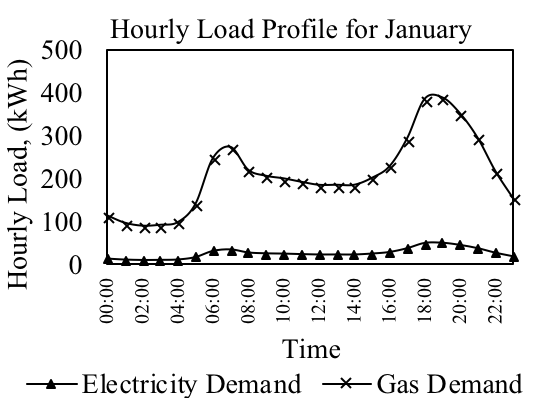
\includegraphics[width=1\hsize]{Figures/LoadProfiles.png}
    \caption{Interpolated hourly load profile for both electricity and gas demand. Adapted from monthly data  \cite{HWES}}
    \label{fig:LoadProfiles}
  \end{figure}
  
  \subsubsection{Resource Data}
  
  Hourly direct and global radiation data is taken from PVGIS \cite{PVGIS} for the location of the building. The same data is also acquired from the Australian Renewable Energy Mapping Infrastructure \cite{AREMI} for a location with stronger irradiance which is used to draw comparisons and conclusions. This data is imported and vectorised in Matlab.
  
  \subsection{Energy Balance}
  
 Equations for PV panels, flat-plate collectors, battery charge/discharge and the two objectives of minimising consumer cost and maximising the CO\textsubscript{2} reduction are required. These are laid out below.
 
\subsubsection{Photovoltaic}

\begin{equation}
E_{PV} = N_{PV} \ A_{PV} \ I_{G} \ \eta_{PV}
\end{equation}
\newline
Where:\newline
E\textsubscript{PV} = Electricity output from the PV array;\newline
N\textsubscript{PV} = Number of PV panels;\newline
A\textsubscript{PV} = Area covered by one PV panel;\newline
I\textsubscript{G} = Global radiation present at the location;\newline
$\eta _{PV}$ = Solar panel efficiency.\newline

Eq. 1 shows the electricity output from the PV array. This equation is based on the panels being horizontal. If the panels were being installed on a tilted roof, this would change.

\subsubsection{Solar Thermal}

\begin{equation}
Q_U = F_R \tau \alpha \ A_{ST} \ I_D \ - \ F_R U_L \ A_{ST} \ (T_{in} - T_{amb})
\end{equation}
\newline
Where:
$Q_U$ = The useful heat energy generated by the array of solar thermal panels;\newline
$F_R \tau \alpha$ = A constant relating to transmittance and absorbance of the panel being used;\newline
$A_{ST}$ = The area covered by one solar thermal panel;\newline
$I_D$ = Direct radiation received by the panels from the sun;\newline
$F_R U_L$ = A constant for the specific panel being used;\newline
$T_{in}$ = Temperature of the fluid within the panel;\newline
$T_{amb}$ = Ambient temperature, 25{\degree}C. \newline

Eq. 2, shows the useful heat output generated by the ST array. This equation is based on a flat plate collector, and therefore is not valid for tube collectors.

\subsubsection{Heat Storage}

if $Q_{U_{n+1} \ > \ Q_{D_{n+1}}}$:

\begin{equation}
Q_{T_{n+1}} = Q_{T_n} \ + (\ Q_{U_{n+1}} \ - \ Q_{D_{n+1}}) 
\end{equation}

Else If $Q_{U_{n+1}} \ < \ Q_{D_{n+1}}$ \newline

\hspace*{15pt} \vspace*{2pt} And $Q_{T_n} \ \geq \ Q_{D_{n+1}} \ - \ Q_{U_{n+1}}$:

\begin{equation}
Q_{T_{n+1}} =Q_{T_{n}} \ + \ (Q_{U_{n+1}} \ - \ Q_{D_{n+1}})
\end{equation}

\hspace*{15pt} Else 
\begin{equation}
Q_{T_{n+1}} = 0
\end{equation}

Else 
\begin{equation}
Q_{T_{n+1}} = Q_{T_{n}}
\end{equation}
\newline
Where:
n = Previous timestep;\newline
n+1 = Current timestep;\newline
$Q_D$ = Heating demand;\newline
$Q_T$ = thermal storage level.\newline
\newline
Eq. 3,4,5 and 6 are for thermal storage. This states that when the useful heat energy generated is larger than the demand, the excess will be stored. If the demand is larger than the generation, then the stored energy will be used to cover the excess demand. 

\subsubsection{Electrical Storage}

if $E_{PV_{n+1} \ > \ E_{D_{n+1}}}$:

\begin{equation}
E_{B_{n+1}} = E_{B_n} \ + (\ E_{PV_{n+1}} \ - \ E_{D_{n+1}}) 
\end{equation}

Else If $E_{PV_{n+1}} \ < \ E_{D_{n+1}}$ \newline

\hspace*{15pt} \vspace*{2pt} And $E_{B_n} \ \geq \ E_{D_{n+1}} \ - \ E_{PV_{n+1}}$:

\begin{equation}
E_{B_{n+1}} =E_{B_{n}} \ + \ (E_{PV_{n+1}} \ - \ E_{D_{n+1}})
\end{equation}

\hspace*{15pt} Else 
\begin{equation}
E_{B_{n+1}} = 0
\end{equation}

Else 
\begin{equation}
E_{B_{n+1}} = E_{B_{n}}
\end{equation}
\newline
Where:
$E_D$ = Electricity demand, W;\newline
$E_B$ = Electricity stored in the Li-Ion batteries;\newline
\newline
Eq. 7,8,9 and 10 describe the electricity storage system. It works in the same way as that of the thermal storage as described previously. 

\subsubsection{Performance Indicators}

\begin{equation}
S = \frac{1}{E_{out} \ s_{PV} + Q_{out} \ s_{ST}}
\end{equation}

\begin{equation}
C = N_{PV} \ c_{PV} \ + \ N_{ST} \ c_{ST} \ + \ c_B \ + \ c_T \ - \ c_s
\end{equation}
\newline
where: 
S = Total $CO_2$ saving in kg; \newline
$E_{out} = s_{PV} \ A_{PV} \ N_{PV} \ I_G  \ \eta_{PV}$;\newline
$Q_{out} = (s_{ST} (F_R \tau \alpha \ A_{ST} \ N_{ST} \ I_D ) \ - \ (F_R U_L \ A_{ST} \ N_{ST} \ (T_{in} - T_{amb})$; \newline
$s_{PV} = 0.482 \ kg \  \frac{CO_2}{kWh}$; \newline
$s_{ST} = 0.24 \ kg \ \frac{CO_2}{kWh}$; \newline
C = The consumer cost; \newline
$c_{PV}$ = Cost per panel \newline %%(210*0.77*1.2); [ref] 
$P_{PV}$ = Rated power output of the PV panel in kW.; \newline %%[ref]
$c_{ST}$ = Cost of the solar thermal panels in £/Unit \newline %%($900); [ref] 900*0.77*1.2
$c_B$ = Cost of the electrical storage system; \newline %%[ref]
$c_T$ = Cost of the heat storage system; \newline %%[ref]
$c_s$ = Total value of savings earned from tariffs. \newline

Eq. 11 and 12 are the performance indicators for the project. Eq. 11 is the total carbon dioxide saving in kg and Eq. 12 is the consumer cost. These two equations are the basis of what the GA is working towards finding the optimal solution to.

\subsection{Genetic Algorithm}

The built in genetic algorithm function within the Global Optimisation Toolbox for Matlab is used. It is tailored to fit the purpose. This program uses the function ‘GAMULTIOBJ’ \cite{GAMULTIOBJ} to perform the genetic algorithm on the multi-objective problem. This built-in function aims to minimise the two specified objectives. It does this through the use of the fitness function and constraint function as well as a specified set of options, including boundary conditions and number of variables.

\subsubsection{Fitness Function (Objective Function)} 
The fitness function takes the input data, and using the two objective function equations, as defined by the performance indicators earlier, calculates two vectors of data. This process is repeated using the new values for the variable.

\subsubsection{Constraint Function}
To ensure the solutions obtained from the genetic algorithm simulation are suitable, a constraint function is required. The constraint function in this case contains 3 separate constraints: The total area covered by both types of panels must not exceed the defined maximum area; the PV panels must meet a specified portion of the total electricity demand; the solar thermal panels must meet a specified portion of the total thermal demand required.

The following three equations are passed through as the constraint function, c:
 
\begin{equation}
N_{PV} \ A_{PV} \ + \ N_{ST} \ A_{ST} \ - \ A_{max}
\end{equation}

\begin{equation}
x E_D \ - \ E_{out}
\end{equation}

\begin{equation}
x Q_D \ - Q_{out}
\end{equation}

where x is the factor of the demand that must be met by the system for the Pareto front.

\subsubsection{Options}

The options function allows for plotting of the results in a Pareto plot, as well as allowing for the passing of all information required by the genetic algorithm. To obtain a sufficient amount of results on the Pareto front, a population size of 200 is implemented. Custom creation, mutation and crossover functions are also passed through using functions created by MathWorks \cite{matlabb}. This allowed for the final values for the number of PV panels, flat-plate collectors, Li-Ion batteries and PCM heat batteries to be given in integer form instead of the default real number format.

\subsection{Constant Values}

There are various constants used throughout the simulation. These values are defined as in Table \ref{Constants}. Depending on the model of the panels the areal, transmittance, absorbance and heat loss coefficient are all subject to change. This simulation only uses one of each panel type and therefore are constant here.

\begin{table}[H]
\caption{Summary of variables and constants with their values and definition.}
\vspace{5pt}
\label{Constants}
\centering
\begin{tabular}{@{}lll@{}}
\toprule
\textbf{Constant} & \textbf{Value} & \textbf{Definition} \\ \toprule
F$_R$U$_L$ & 3.4 & Heat loss coefficient \\ \midrule
F$_R$$\tau$$\alpha$ & 0.726 & Transmittance/Absorbance \\ \midrule
T$_{in}$ & 70\degree C & Temperature of collector. \\ \midrule
T$_{amb}$ & 25\degree C & Ambient temperature. \\ \midrule
A$_{ST}$ & 2.5m$^2$ & Flat-plate collector area. \\ \midrule
A$_{PV}$ & 1.91m$^2$ & PV panel area. \\ \midrule
A$_{max}$ & 1600m$^2$ & Maximum areal space. \\ \midrule
V$_B$ & 0.13m$^3$  & Li-Ion battery volume. \\ \midrule
V$_{TB}$ & 0.26m$^3$ & Heat battery volume. \\ \midrule
s$_{PV}$ & $0.482 \ kg \  \frac{CO_2}{kWh}$ & CO$_2$ savings from PV \cite{britgas}. \\ \midrule
s$_{ST}$ & $0.24 \ kg \  \frac{CO_2}{kWh}$ & CO$_2$ savings from ST \cite{britgas}. \\ \midrule
c$_{PV}$ & £186 & Cost of a PV panel \cite{irenaB}. \\ \midrule
c$_{ST}$ & £835 & Cost of a ST panel \cite{ecodirect} \\ \midrule
c$_B$ & £1540 & Cost of electrical storage \cite{irena}. \\ \midrule
c$_T$ & £2100 & Cost of thermal storage \cite{sunamp}. \\ \midrule
c$_s$ &£0.635/kW & UK gen. tariff \cite{EST1} \cite{EST2}. \\ \midrule
\end{tabular}
\end{table}

\subsection{Program Flow Chart}

The flow chart can be seen in Appendix A. It details the method by which the genetic algorithm will function. It takes the inputs of resource data, component data, constraints, boundaries, fitness function and options data and then implements the algorithm. Once it has completed the process, a check is done by the algorithm to see if the criteria have been met, if the criteria are not met, the algorithm will repeat until the solution is obtained.




 
\section{Results and Discussion}

To look at the effects of the demand on the output, the demand data is scaled up and down to allow a comparison between high-use years and low-use years. Similarly, sensitivity analysis is performed on the location, to see how important the location can be on the performance.

\subsection{Case 1: Scotland }

Case 1 uses the Lord Thomson building at Heriot-Watt University as the demand. The resource data used is for Edinburgh, Scotland. Three scenarios are simulated which include the base case, where the demand is unchanged, a reduced demand scenario, where the demand is reduced by 50\% and a third scenario where the demand is reduced by 90\%. 

\subsubsection{Pareto Front}

\begin{figure}[H]
	\centering
    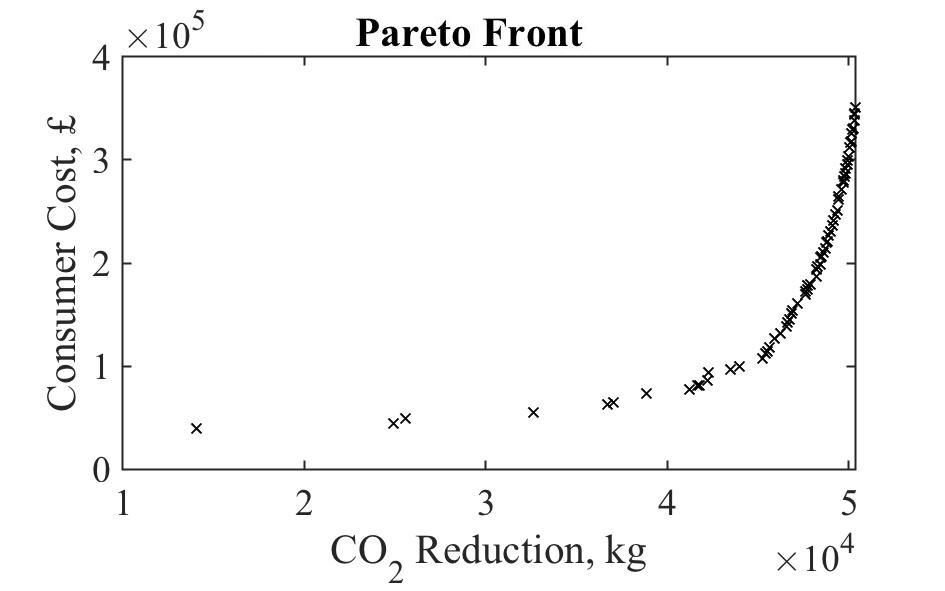
\includegraphics[width=\columnwidth]{Figures/ParetoBase.jpg}
    \caption{The Pareto front for the base case scenario. The two optimised objective functions are plotted with consumer cost on the y-axis and $co_2$ reduction on the x-axis.}
    \label{fig:ParetoBase}
\end{figure}

Fig. \ref{fig:ParetoBase} shows the pareto front obtained from the simulation. It shows a trend of increased CO$_2$ reduction leading to an increase in the consumer cost. The consumer cost is being minimised while the CO$_2$ reduction is being maximised. The range of solutions is from £50,000 to £440,000 for consumer cost. The CO$_2$ reduction ranges from approximately 15,000 kg to 50,000 kg. This is the base case pareto front, where it is not possible to get anywhere near meeting the demand. In this case the constraint on the minimum acceptable solution is not set. This is due to two factors: The first being a high demand for the building; The second is the low strength of the solar insolation coupled with the lack of roof space required at that strength. When a value is set for the constraint, the simulation cannot run.

\begin{table}[H]
\caption{Four selected solutions on the Pareto front ranging from minimum to maximum points for Case 1.}
\vspace{5pt}
\label{case1}
\centering
\begin{tabular}{@{}llll@{}}
\toprule
\begin{tabular}{@{}l@{}}{\textbf{CO$_2$}} \\ \textbf{Reduction, kg}\end{tabular} 
& \begin{tabular}{@{}l@{}}{\textbf{Consumer}} \\ \textbf{Cost, £}\end{tabular} 
& \begin{tabular}{@{}l@{}}{\textbf{PV/ST}}  \\ \textbf{Panels}\end{tabular}
& \begin{tabular}{@{}l@{}}{\textbf{Li-ion/Heat}} \\ \textbf{Batteries}\end{tabular} \\ \toprule
50,000 & 351,000 & 517/245 & 46/27 \\ \midrule
48,000 & 161,000 & 708/80 & 29/7 \\ \midrule
37,000 & 63,000 & 494/8 & 14/4 \\ \midrule
14,000 & 40,000 & 101/20 & 1/8 \\ \midrule
\end{tabular}
\end{table}

Table \ref{case1} gives four selected solutions on the pareto front. These solutions are the maximum and minimum points on the front and one point at each side of the curve. The values vary greatly, but all lie on the pareto front and therefore are classed as pareto optimal solutions.



\subsubsection{Optimised Objectives vs Simulation Variables}

\begin{figure}[H]
	\centering
    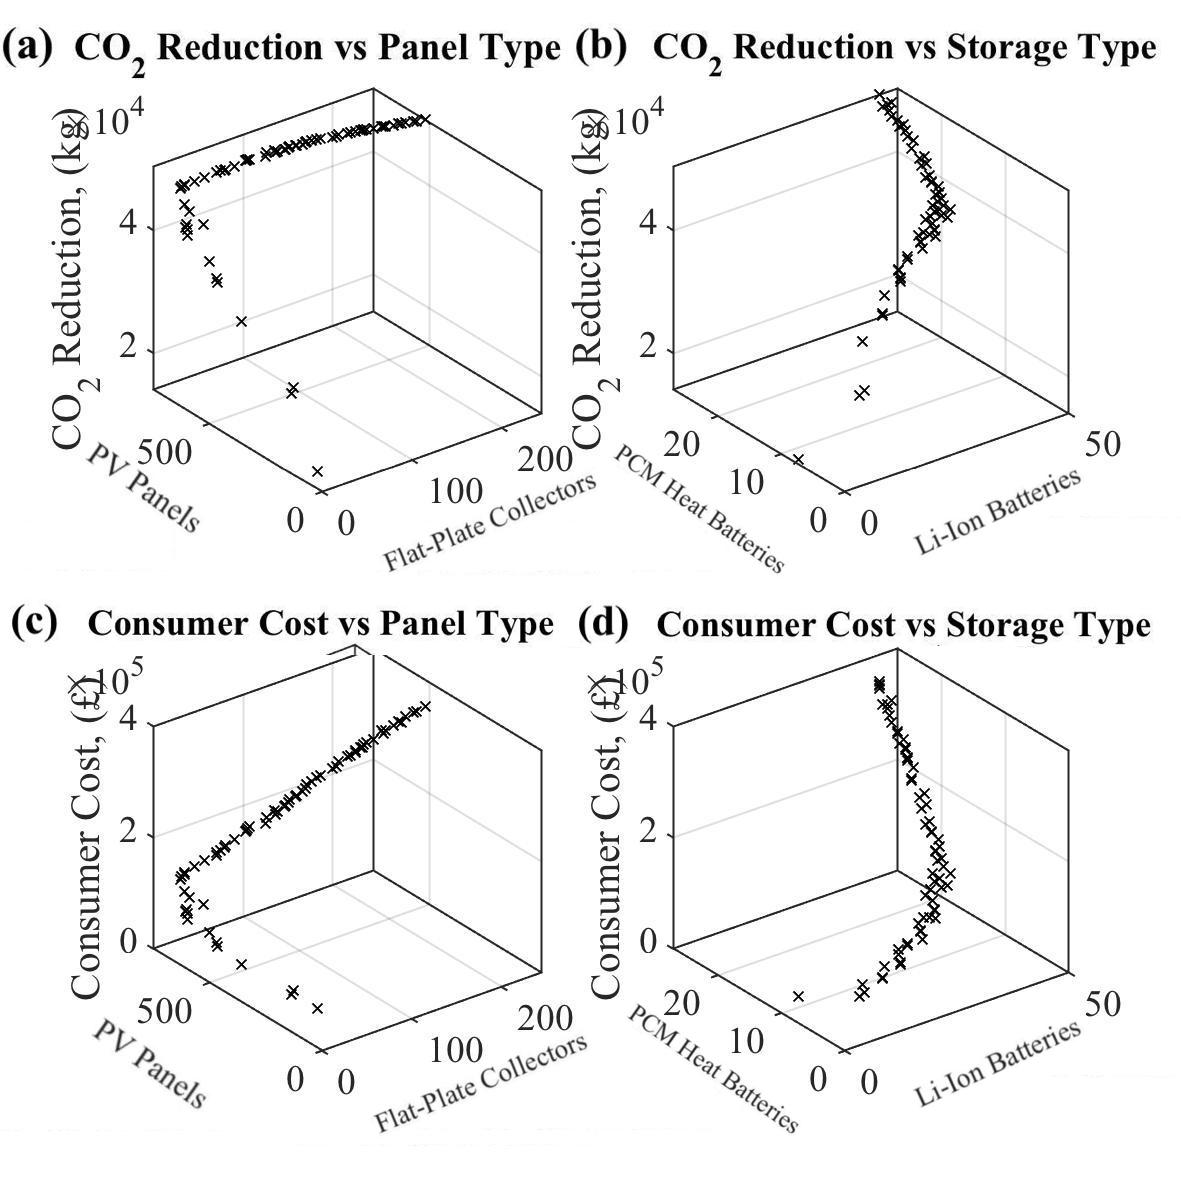
\includegraphics[width=235pt]{Figures/RedAndCostVsPanelsAndStorageBase1.jpg}
    \caption{3-Dimensional plots of the optimised objectives with respect to the the simulation variables. (a) Panel type vs CO$_2$ reduction, (b) Storage type vs CO$_2$ reduction, (c) Panel type vs consumer cost, and (d) Storage type vs consumer cost}
    \label{fig:ObjectivesVsPanelsVsStorage}
\end{figure}
  
  Fig. \ref{fig:ObjectivesVsPanelsVsStorage} is the amount of PV and solar thermal panels used for each scenario on the Pareto front plotted against the CO$_2$ reduction. This shows that the main factor in reducing the amount of CO$_2$ produced is by increasing the number of PV panels. It increases the reduction in CO$_2$ from 30,000 kg at 300 PV panels to 45,000 kg at 800 PV panels. As the amount of flat plate collectors increases, the reduction in CO$_2$ emissions is not greatly affected. This is due to the fact that, despite a reduction of 0.24 kg CO$_2$/kWh generated, the direct solar insolation present is not strong enough to produce energy for a large portion of the year. The flat plate collectors contribute approximately 5000 kg of reduced CO$_2$ emissions at 200 collectors. Figure 3(c) shows the effect on consumer cost of the various combinations of panels. It can be seen that the flat plate collectors are a larger outlay. This is expected as due to the low amount of energy produced by each flat plate collector, the tariff (see \ref{Constants}) from generating energy is unable to have a large effect on the outlay. Whereas with PV panels, the initial outlay is offset by the tariff on generating electricity in this way. The overall consumer cost ranges from approximately £30,000 up to £400,000. Most of the solutions occur between £100,000 and £400,000 consumer cost. Fig. 3(b) and Fig. 3(d) detail the storage means with each of the objective functions. In general, the more of each type of battery in the system, the higher the cost and the higher the reduction in emissions. This is in line with the amount of each type of panel being used to generate the energy. 
  
\subsubsection{Storage Performance}

\begin{figure}[H]
	\centering
    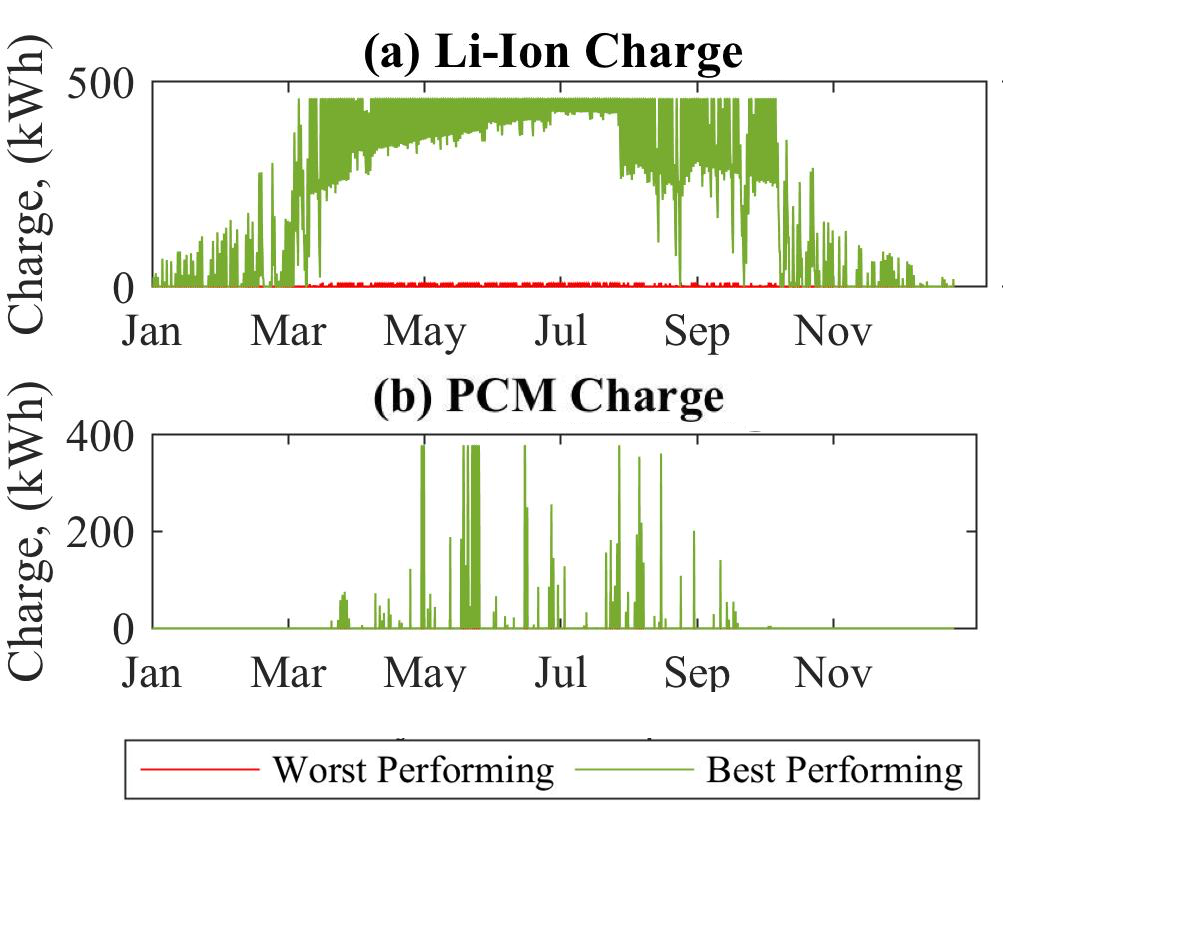
\includegraphics[width=1.1\columnwidth]{Figures/StorageLevels.png}
    \vspace*{-15mm}
    \caption{(a) Hourly charge level of the Li-Ion battery array in kWh with respect to time and (b) PCM heat battery array in kWh with respect to time.}
    \label{fig:StorageLevels}
\end{figure}
  
Fig. \ref{fig:StorageLevels}(a) shows the best and worst performing Li-Ion battery scenarios. The best-case scenario, in green, shows a maximum level of 420 kWh. It remains above zero, i.e. the demand is being met at all times from April until mid-October, apart from on two short occasions in September and October. Between January and March, and November and December the battery bank level depletes to zero on numerous occasions. This indicates that not enough energy is being produced to meet the demand. This is also the circumstance for the worst case, shown in red. The worst case is unable to provide any energy to meet the demand outwith the months of March to October.
 
In the case of the best and worst performing scenarios for the PCM heat battery, shown in Fig. \ref{fig:StorageLevels}(b), the worst performing scenario results in zero kWh of thermal energy being stored at any point. The best performance is still inadequate. This is due to the poor direct insolation at the location. The maximum level of the battery bank is only reached on very few occasions during the year and each time it reaches maximum capacity, the stored energy is then utilised soon after in order to meet the demand.

\begin{figure}[H]
	\centering
    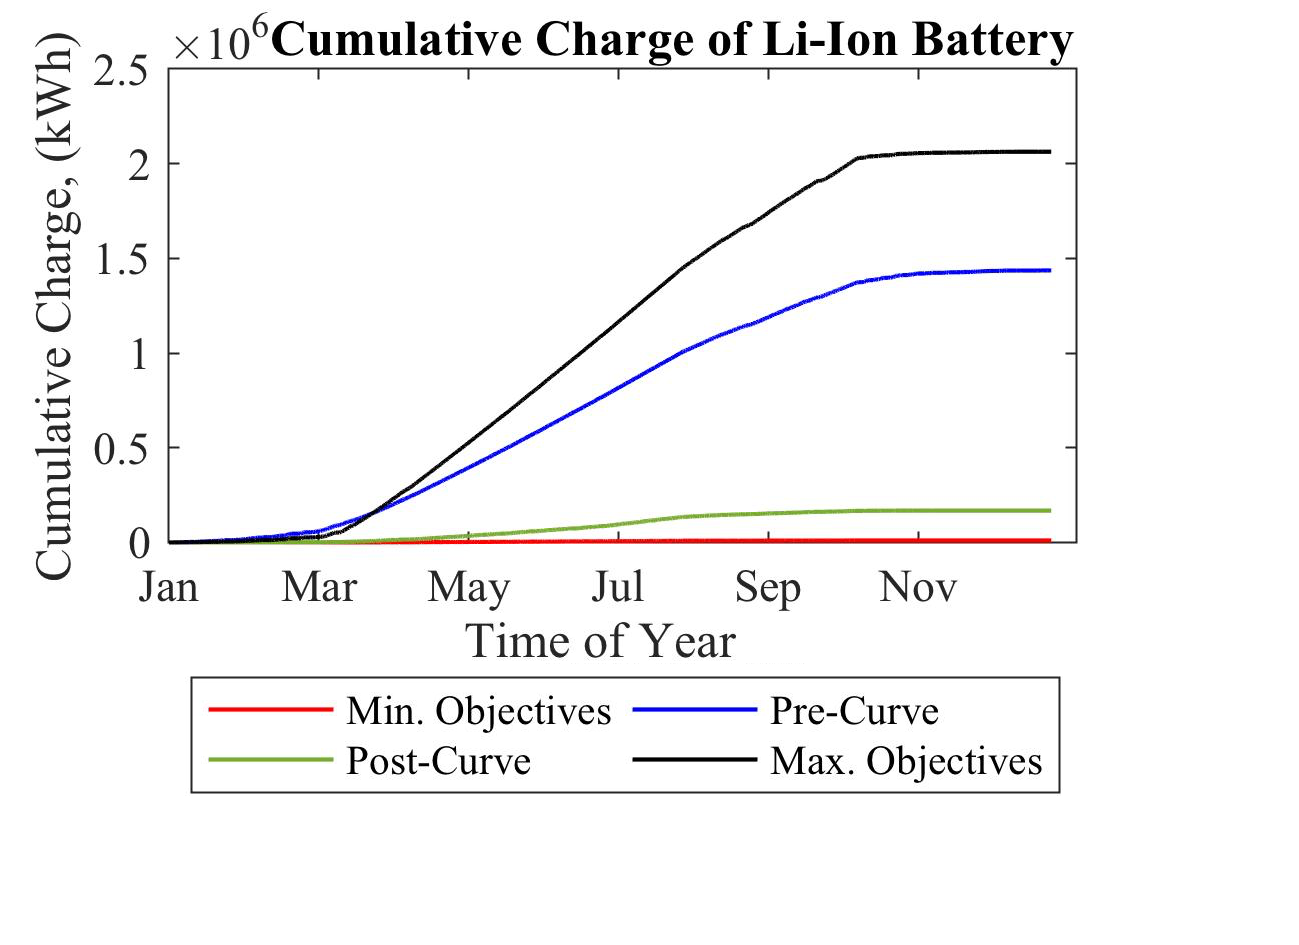
\includegraphics[width=255pt]{Figures/CumChargeBat.png}
    \vspace*{-15mm}
    \caption{Four scenarios for the cumulative charge of the Li-Ion battery array with respect to time. Each line represents one point on the Pareto front from lowest consumer cost to highest consumer cost.}
    \label{fig:CumChargeBat}
\end{figure}
 
 \begin{figure}[H]
	\centering
    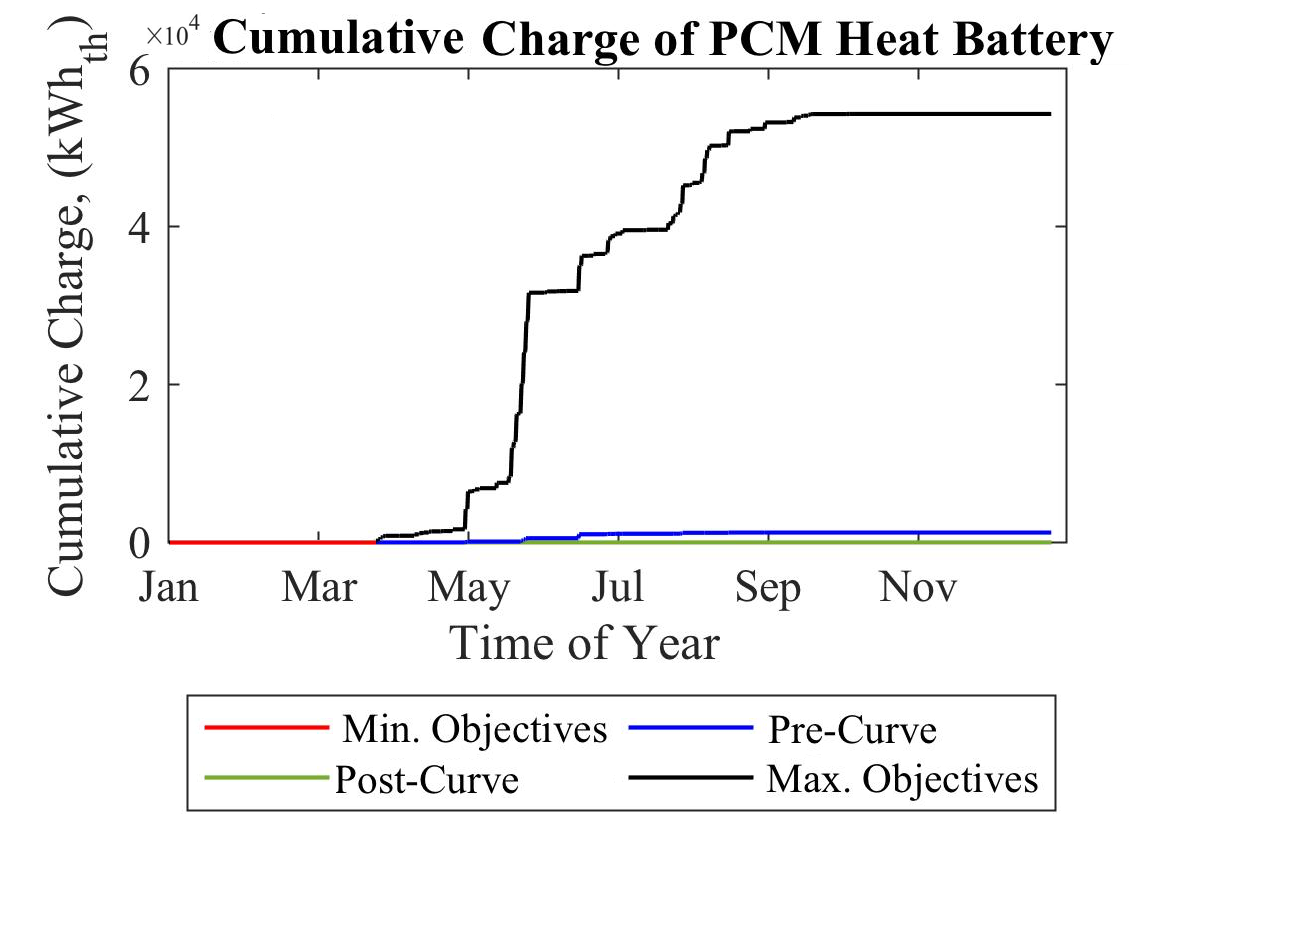
\includegraphics[width=255pt]{Figures/CumChargeHBat.png}
    \vspace*{-15mm}
    \caption{Four scenarios for the cumulative charge of the PCM heat battery array with respect to time. Each line represents one point on the Pareto front from lowest consumer cost to highest consumer cost.}
    \label{fig:CumChargeHBat}
\end{figure}

Fig. \ref{fig:CumChargeBat} and Fig. \ref{fig:CumChargeHBat} show the cumulative charge of the Li-Ion battery array and PCM heat battery array with respect to time. For both, the best scenario is when the maximum consumer cost solution is used. This is due to a higher amount of panels and batteries being used in this case and as such, more energy is generated and stored. The Li-Ion battery array reaches its highest cumulative point at 2 GWh in the highest consumer cost scenario. At minimum consumer cost, the storage is almost zero throughout the simulation as there is minimal storage capacity on site. Similarly for the PCM heat battery array, three of the four scenarios indicate minimal thermal energy storage. The best case peaks at 54 MWh of cumulative storage.

\subsubsection{Areal Coverage}
\vspace*{1mm}
\begin{figure}[H]
	\centering
    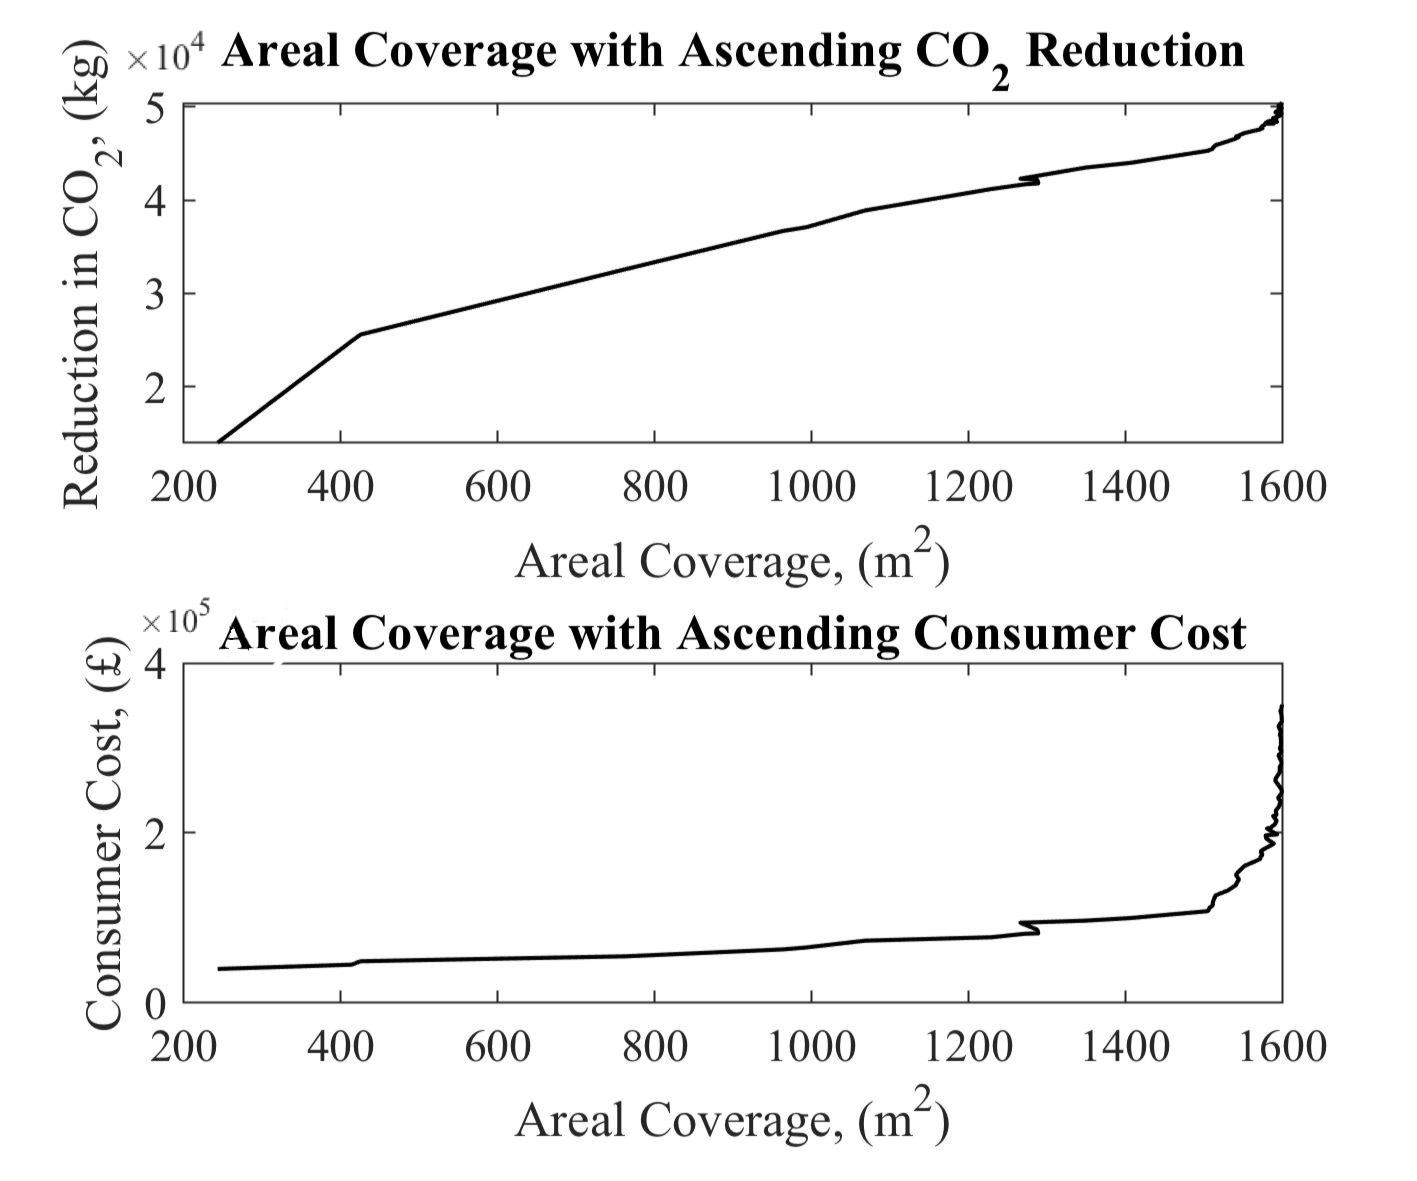
\includegraphics[width=245pt]{Figures/ArealCoverage.jpg}
    \caption{Areal coverage of panels on roof space with respect to the two objective functions.}
    \label{fig:ArealCoverage}
\end{figure}

Fig. \ref{fig:ArealCoverage} indicates that the higher the value of the objective functions is, the more areal space is covered by panels. The top graph indicates a reasonably steady climb in CO$_2$ reduction with an increase in areal coverage. The bottom graph has a steady inclination in consumer cost up until around 1500m$^2$, where there is a sharp increase in the consumer cost for a relatively small increase in areal coverage. This indicates that at higher areal coverage, a larger amount of storage is required and thus a large spend on batteries is required. It is also noticeable that the maximum area of 1600m$^2$ is not exceeded and therefore the constraint on the number of panels allowed (or maximum area allowed) is limiting the solution space as intended.

\subsubsection{Sensitivity Analysis}

Sensitivity analysis is performed on the Pareto front by altering the demand from the base case to 50\% and 10\%.

\begin{figure}[H]
	\centering
    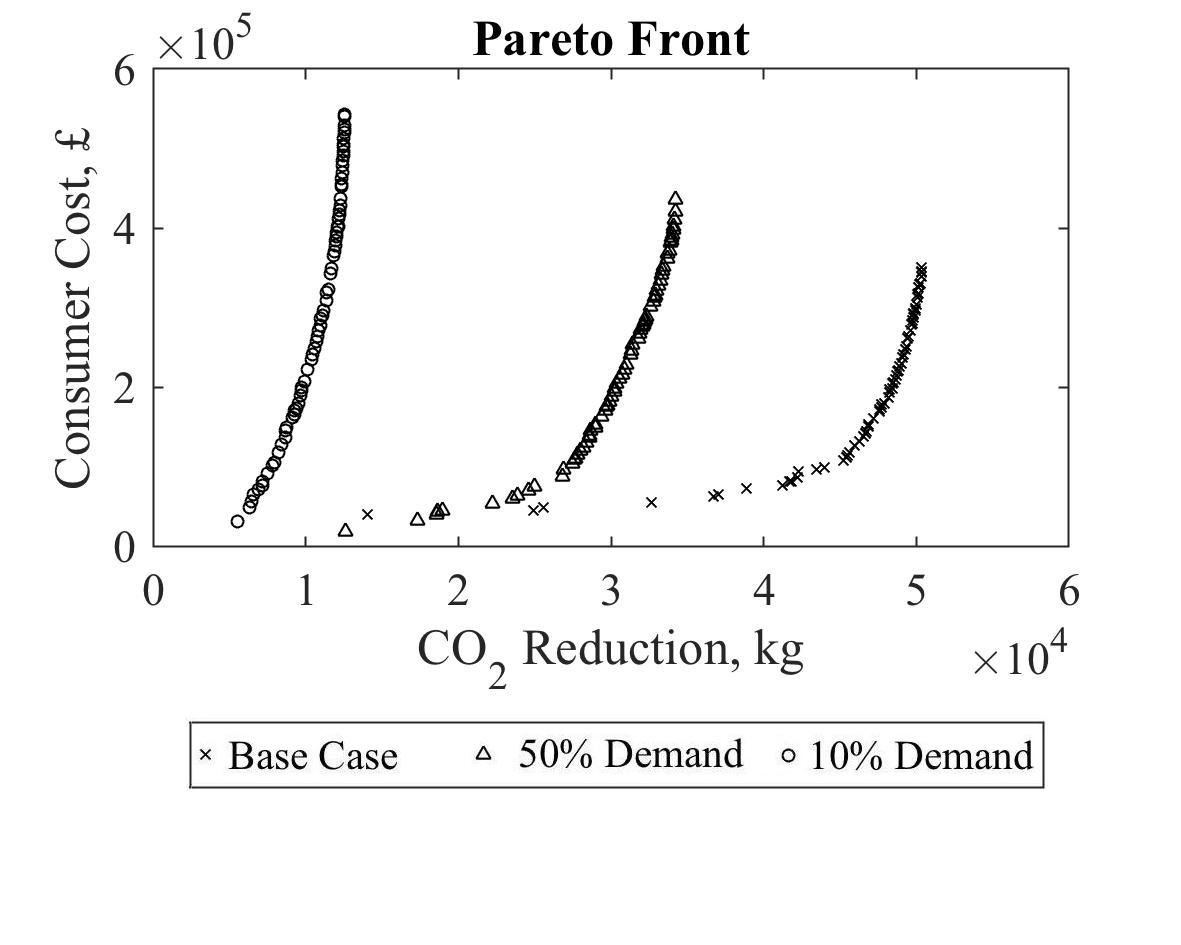
\includegraphics[width=\columnwidth]{Figures/ParetoSens1.jpg}
    \vspace*{-15mm}
    \caption{Sensitivity of the Pareto front to change in the electrical and thermal energy demand. Base case, 50\% and 10\% demand scenarios are shown.}
    \label{fig:ParetoSens}
\end{figure}
  
Fig. \ref{fig:ParetoSens} shows the effect of varying the demand on the Pareto front. The base case, indicated by X shows the same data as was described previously. When the demand is halved, the Pareto front shifts to the right. The trend is very similar to the base case and therefore the system is reasonably robust. However, when the demand is cut to just 10\%, the Pareto front shifts greatly to the right and the curve is different in shape. It transitions more smoothly and gradually than that of the base case and halved demand case. The difference is most evident in the middle of the curve where it is greatly different. This indicates that the system can handle small changes in the demand but would become inaccurate if the demand is greatly changed from the values it is designed for.

\subsection{Case 2: Australia}

Case 1 uses the Lord Thomson building at Heriot-Watt University as the demand. The resource data used is for Perth, Australia. Three scenarios are simulated which include the base case, where the demand is unchanged, a reduced demand scenario, where the demand is reduced by 20\% and an increased demand scenario where the demand is increased by 20\%.  This case allows for results to be seen where solar-thermal is a viable solution.

\subsubsection{Pareto Front}

\begin{figure}[H]
	\centering
    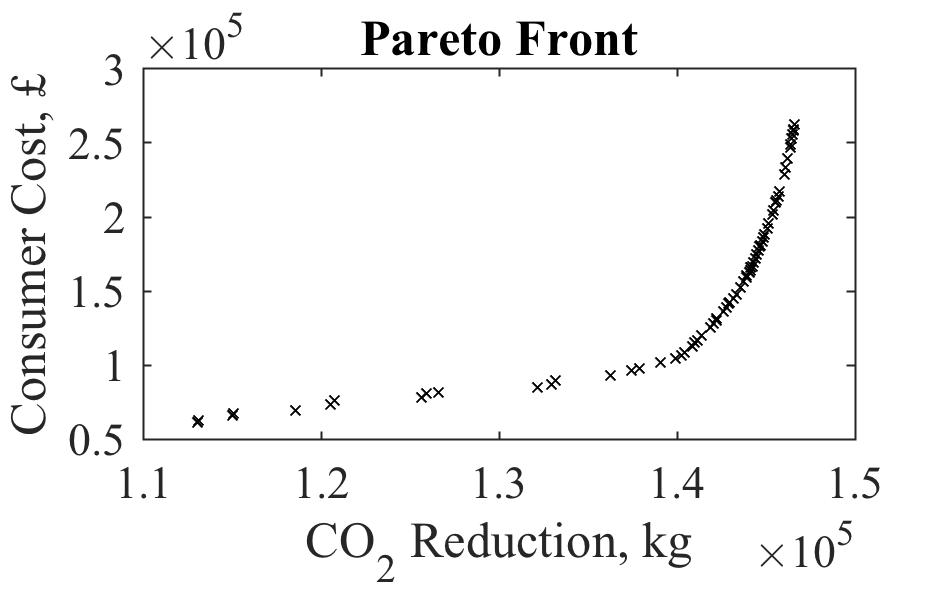
\includegraphics[width=0.95\columnwidth]{Figures/ParetoFront2.jpg}
    \caption{The Pareto front for the case 2 base scenario. The two optimised objective functions are plotted with consumer cost on the y-axis and CO$_2$ reduction on the x-axis.}
    \label{fig:ParetoFront2}
\end{figure}

Fig. \ref{fig:ParetoFront2} shows the Pareto front obtained from the simulation of case 2. The range of solutions is from £60,000 to £250,000. The CO$_2$ reduction ranges from approximately 105,000 to 145,000 kg. In this case, the constraint on the minimum acceptable solution is set to 50\% of the total demand. Since the resource has been changed, the amount of energy generated can be greatly increased, thus allowing for a more limiting constraint which results in a smaller range in the solution. The reduction in CO$_2$ starts much higher than that of case 1 as there is a larger solar radiation available and less allowance for variance in the number of panels due to the constraint of meeting 50\% of the total demand.

\begin{table}[H]
\caption{Four selected solutions on the Pareto front ranging from minimum to maximum points for Case 2.}
\vspace{5pt}
\label{case2}
\centering
\begin{tabular}{@{}llll@{}}
\toprule
\begin{tabular}{@{}l@{}}{\textbf{CO$_2$}} \\ \textbf{Reduction, kg}\end{tabular} 
& \begin{tabular}{@{}l@{}}{\textbf{Consumer}} \\ \textbf{Cost, £}\end{tabular} 
& \begin{tabular}{@{}l@{}}{\textbf{PV/ST}}  \\ \textbf{Panels}\end{tabular}
& \begin{tabular}{@{}l@{}}{\textbf{Li-ion/Heat}} \\ \textbf{Batteries}\end{tabular} \\ \toprule
147,000 & 262,000 & 253/441 & 51/38 \\ \midrule
143,000 & 147,000 & 382/315 & 26/38 \\ \midrule
133,000 & 90,000 & 440/259 & 13/36 \\ \midrule
113,000 & 61,500 & 456/245 & 2/35 \\ \midrule
\end{tabular}
\end{table}

Table \ref{case2} gives four selected solutions on the Pareto front. These solutions range from the maximum to minimum points on the pareto front. Each is an optimised solution to the problem which lies on the front.

\subsubsection{Optimised Objectives vs Simulation Variables}

\begin{figure}[H]
	\centering
    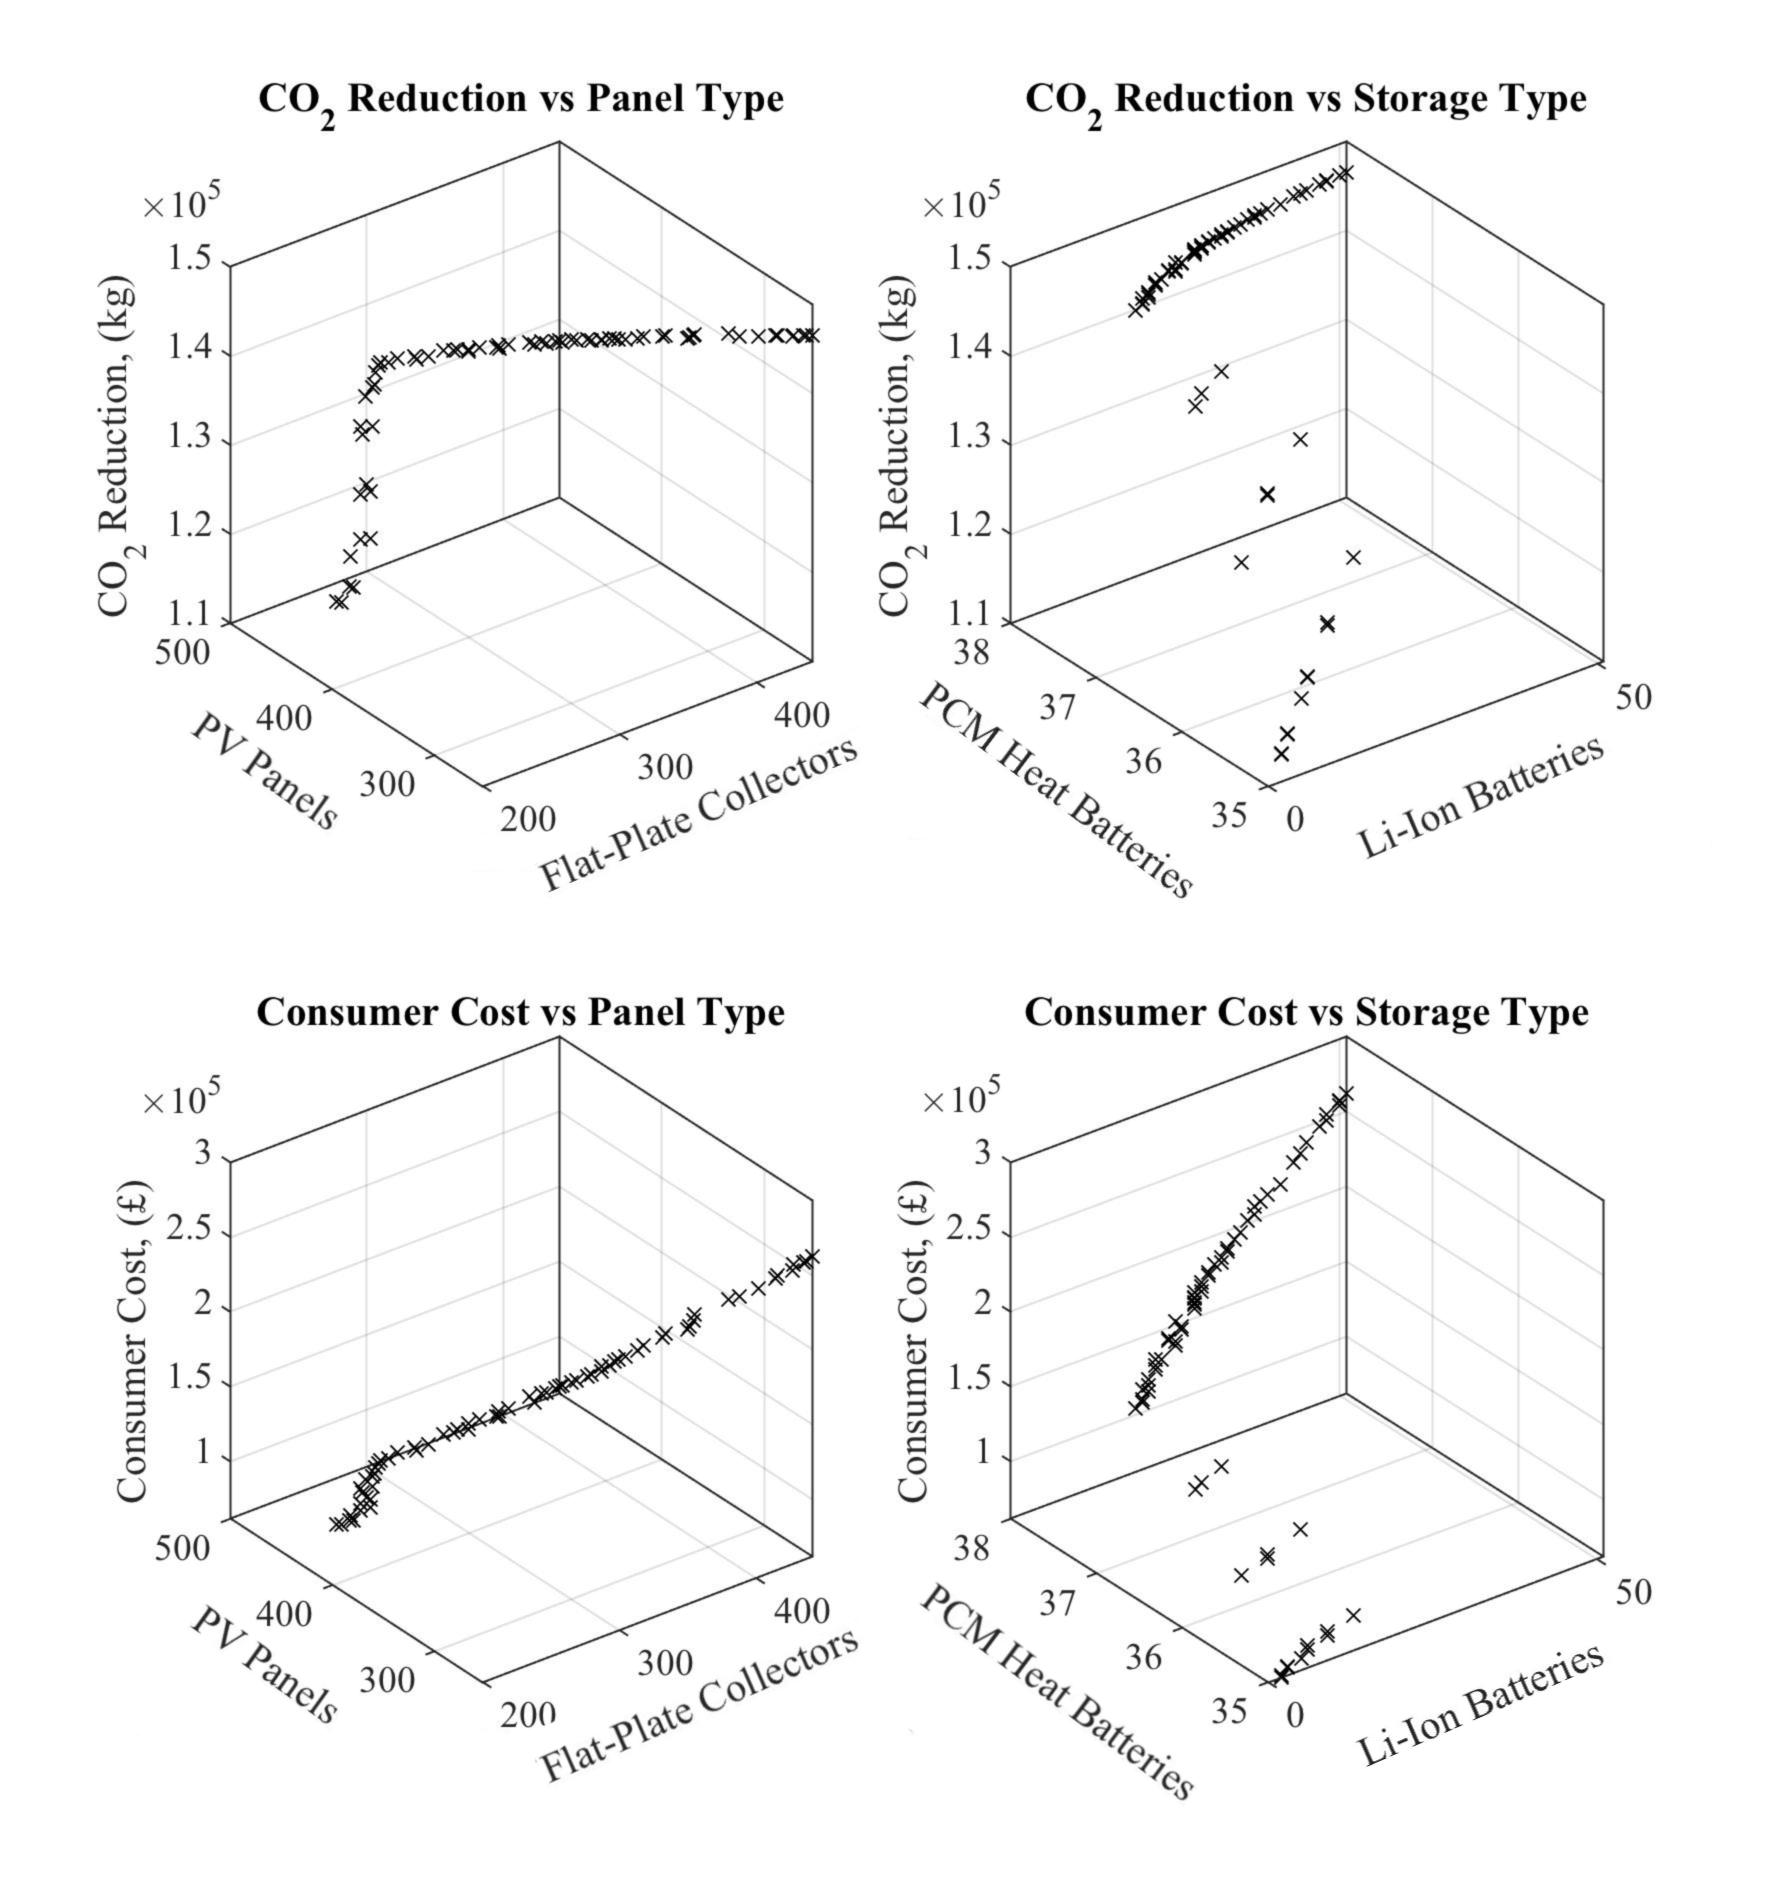
\includegraphics[width=\columnwidth]{Figures/RedAndCostVsPanelsAndStorage2.jpg}
    \caption{3-Dimensional plots of the optimised objectives with respect to the the simulation variables. (a) Panel type vs CO$_2$ reduction, (b) Storage type vs CO$_2$ reduction, (c) Panel type vs consumer cost, and (d) Storage type vs consumer cost}
    \label{fig:ObjectivesVsPanelsVsStorage2}
\end{figure}

Fig. \ref{fig:ObjectivesVsPanelsVsStorage2} shows the reduction in CO$_2$ emissions with respect to PV panels and flat plate collectors. The number of panels is more restricted in this case and varies from 300-500 and 250-450 for PV and flat-plate collectors respectively. The highest reduction in CO$_2$ emissions (approximately 145,000 kg) is present when the number of flat-plate collectors is maximised. Similarly, Fig. \ref{fig:ObjectivesVsPanelsVsStorage2}(c) shows the consumer cost with respect to the number of PV panels and flat plate collectors respectively. The trend is very similar to that of the CO$_2$ reduction, indicating that the consumer cost will peak at a higher ratio of flat plate collectors to PV panels. However, as the amount of PV panels is increased, the consumer cost is reduced. This is due to the generation tariff on PV panels. In reality, this tariff and resource would not occur together. Fig. \ref{fig:ObjectivesVsPanelsVsStorage2}(b) and Fig. \ref{fig:ObjectivesVsPanelsVsStorage2}(d) show the CO$_2$ reduction and consumer cost with respect to each storage method. The simulation is heavily weighted towards a set amount of PCM heat batteries as in order to meet the demand, this storage method is required in large quantities. The variation in Li-Ion batteries is from 0-50, indicating more leniency in electricity storage. It can be seen that as the amount of batteries in the system increases, the consumer cost will increase. Similarly, The CO$_2$ reduction generally increases with the amount of batteries. However, this is due to the increased generation (thus increased reduction in emissions) and not due to the amount of batteries in the system.
  
\subsubsection{Storage Performance}

\begin{figure}[H]
	\centering
    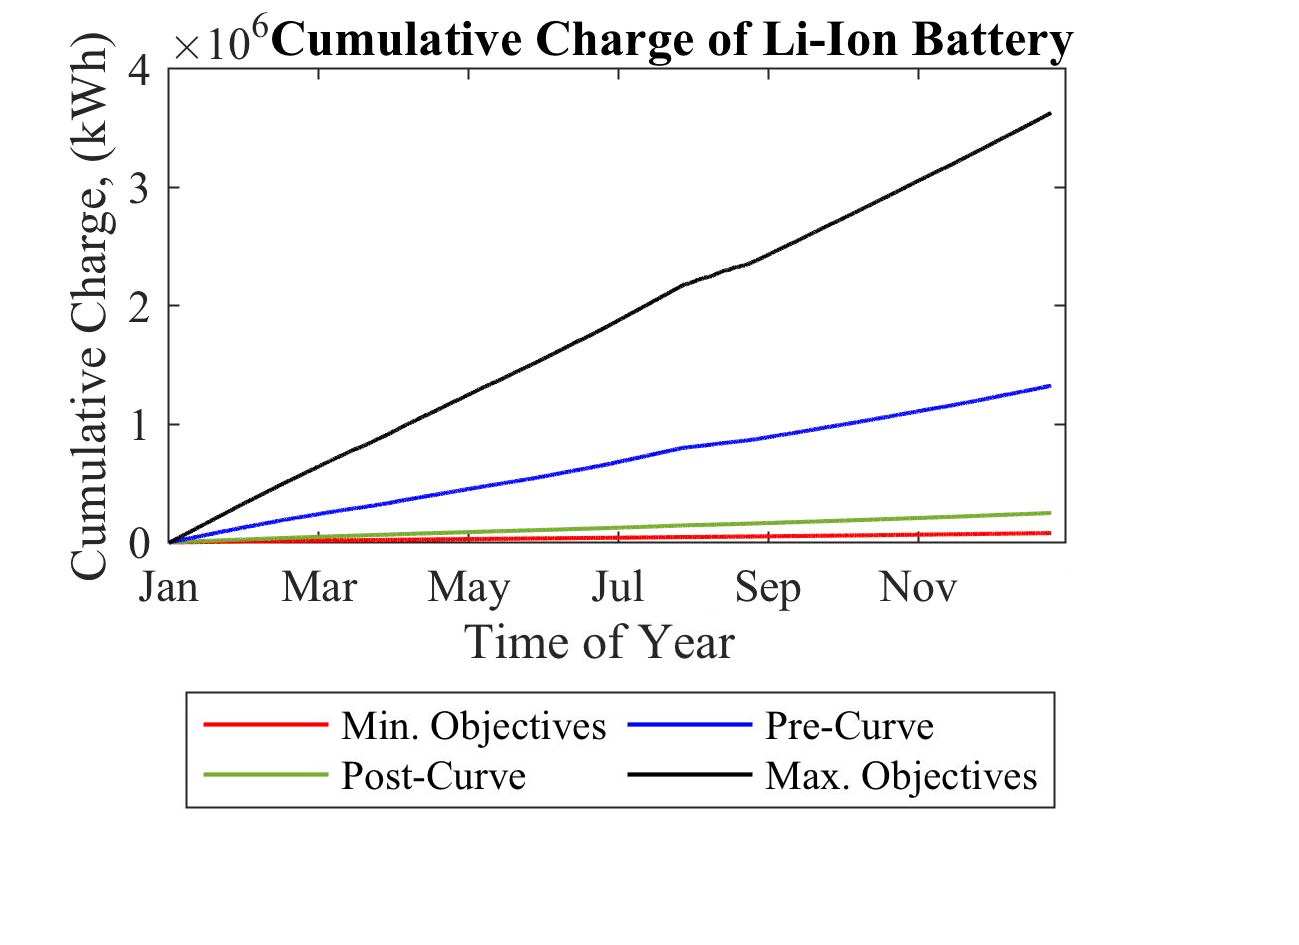
\includegraphics[width=1.12\columnwidth]{Figures/CumBat2.png}
    \caption{Four scenarios for the cumulative charge of the Li-Ion battery array with respect to time. Each line represents one point on the Pareto front from lowest consumer cost to highest consumer cost.}
    \label{fig:CumBat2}
\end{figure}
 
 \begin{figure}[H]
	\centering
    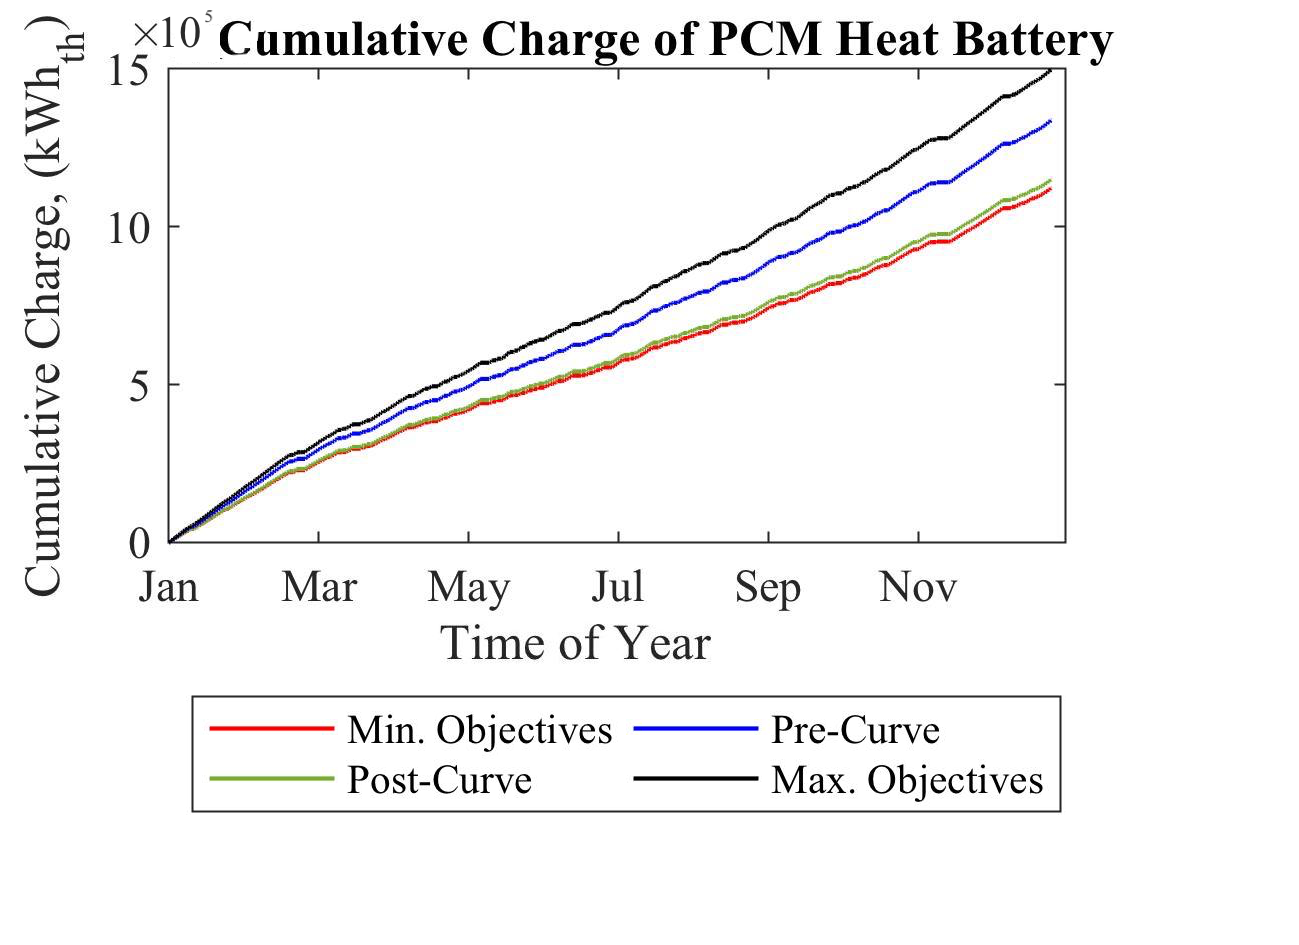
\includegraphics[width=1.12\columnwidth]{Figures/CumHBat2.png}
    \caption{Four scenarios for the cumulative charge of the PCM heat battery array with respect to time. Each line represents one point on the Pareto front from lowest consumer cost to highest consumer cost.}
    \label{fig:CumHBat2}
\end{figure}


Fig. \ref{fig:CumBat2} and Fig. \ref{fig:CumHBat2} show the cumulative charge of the battery arrays for both electrical and thermal storage. In this case, the same trend as case 1 is shown in that as the consumer cost is increased (and reduction in CO$_2$ is also increased) the performance of the storage is also increased. For the Li-Ion battery array, 
the cumulative charge reaches a maximum level of 3.5 GWh and the PCM heat battery array reaches 1.5 GWh of thermal storage. All four scenarios for the PCM heat battery increase linearly throughout the year and even in the case of the lowest consumer cost scenario, there is still a cumulative charge of 1 GWh thermal energy stored. This indicates that when there is a high solar radiation present, the simulation will lean towards maximising the solar thermal potential. In both types of storage, the maximum is higher than that of case 1.

\subsubsection{Areal Coverage}

\begin{figure}[H]
	\centering
    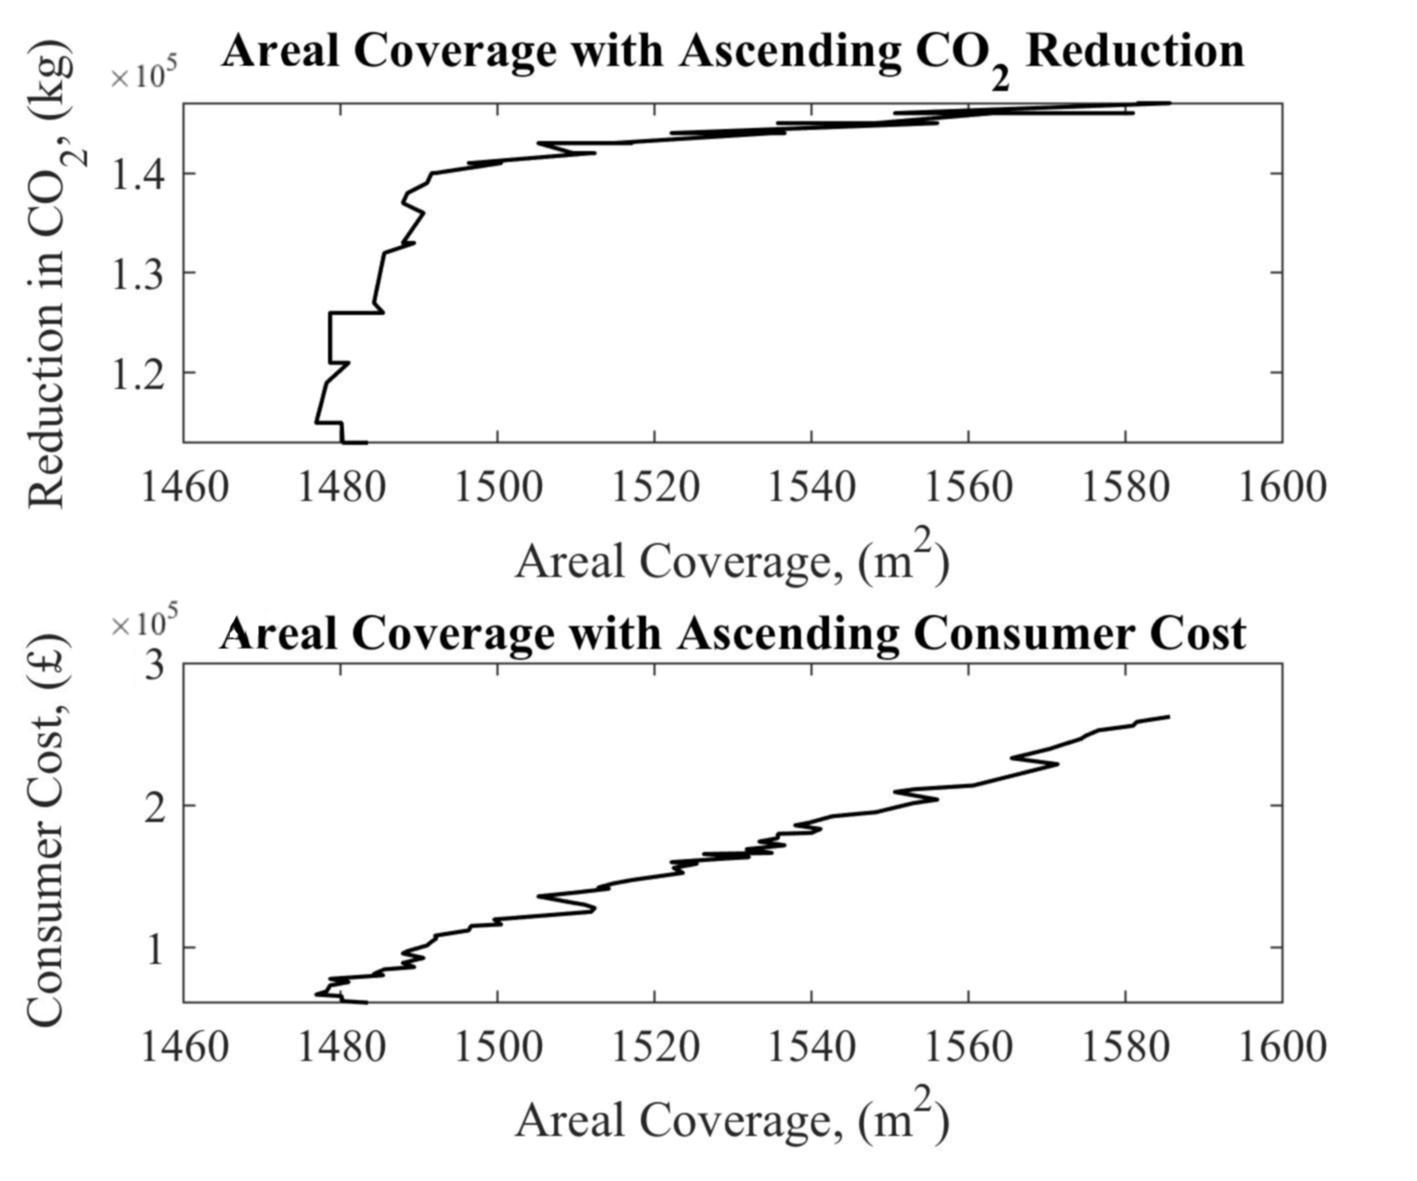
\includegraphics[width=\columnwidth]{Figures/ArealCoverage2.jpg}
    \caption{Areal coverage of panels on roof space with respect to the two objective functions for case 2}
    \label{fig:ArealCoverage2}
\end{figure}

Fig. \ref{fig:ArealCoverage2} indicates that the higher the value of the objective functions is, the more areal space is covered by panels. This trend is visible but in this case there is much more variation. The areal coverage covers a much shorter range of areas for case 2. This is due to the demand constraint meaning a minimum area of around 1480m$^2$ being required. Since the range is smaller, the small changes in the two objective functions are more noticeable. However, the trends are still similar in nature to that of case 1. The jagged nature of the line in the lower graph indicates that despite an increase in the consumer cost, the areal coverage can go down. This is due to the increased amount of storage being used in order to meet the requirements. The maximum area of 1600m$^2$ is not reached for this case as it peaks at 1585m$^2$. This 15m of remaining areal space would only be able to include approximately 7 panels of either type and therefore does not impact the result greatly.
  
\subsubsection{Sensitivity Analysis}

\begin{figure}[H]
	\centering
    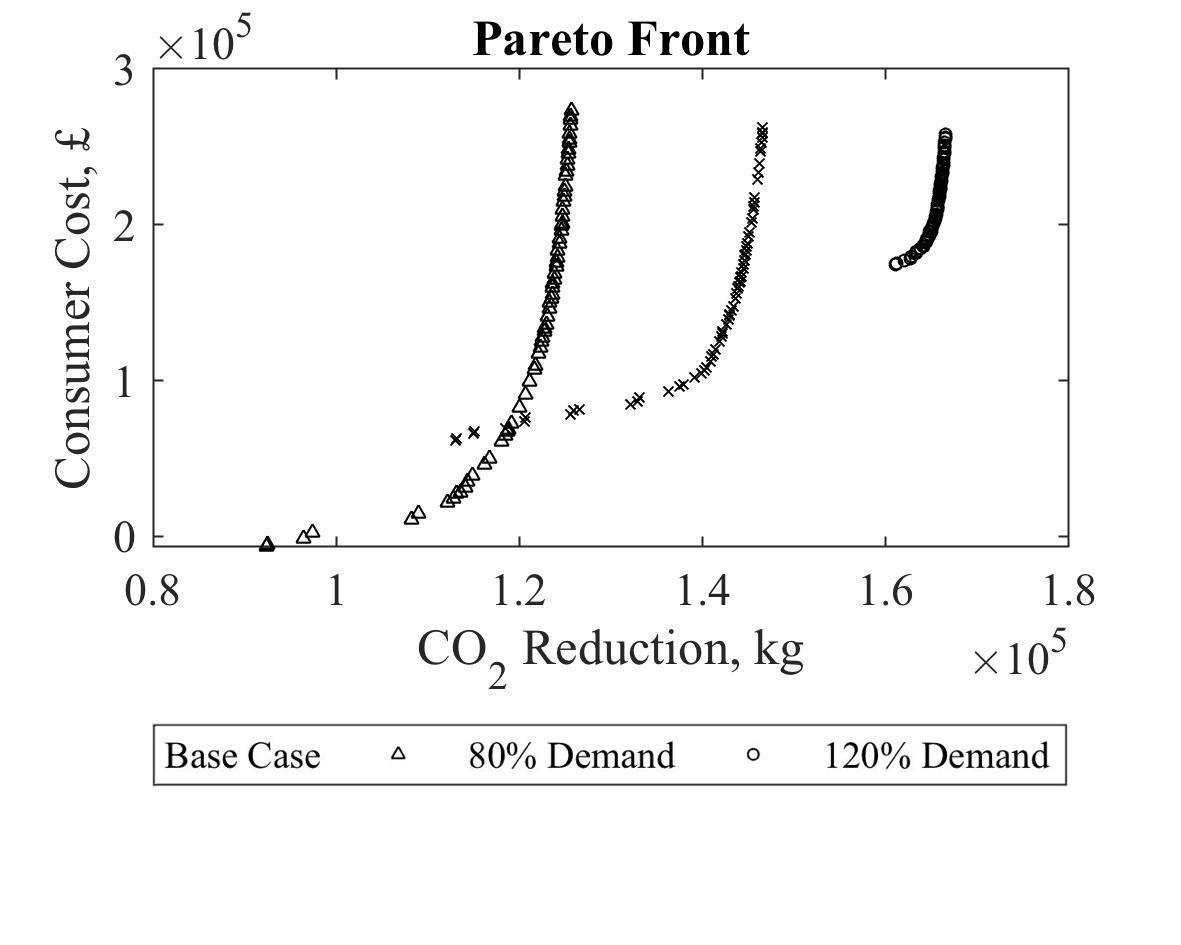
\includegraphics[width=\columnwidth]{Figures/ParetoSens2.jpg}
    \caption{Sensitivity of the Pareto front to change in the electrical and thermal energy demand. Base case, +20\% and -20\% demand scenarios are shown.}
    \label{fig:ParetoSens2}
\end{figure}

Fig. \ref{fig:ParetoSens2} shows the sensitivity of the Pareto front for case 2 when the demand is varied. In this case, the demand has been varied +/- 20\%. It is evident that this change in demand has a large effect on the curve. An increase in the demand of 20\% shifts the curve to the left. It also curves round much earlier than that of the base case, indicating that in this scenario, the solution is not robust. Similarly, a decrease in the demand of 20\% shifts the curve to the right. The spread of solutions is much wider in this case as the program has more room to change. This results in a smoother transition in the curve. In summary, it can be stated that any change in the demand will greatly affect where optimal solutions lie, and therefore use of the model in practice should be limited to scenarios in which there is a high confidence in the demand, resource and other contributing factors.


\section{Conclusion and Recommendations}

In conclusion, this paper has developed a program to optimise a system of PV panels, flat-plate collectors, Li-Ion batteries and PCM heat batteries. This has been achieved through the use of a genetic algorithm to obtain a set of optimised solutions called the Pareto front. A review of literature on the subject has been conducted into solar technologies on rooftops and mathematical optimisation methods in order to gain an insight into ways of tackling the problem. The methodology developed is shown in detail with all equations and variables given, including a flow chart indicating the steps required in order to optimise the solutions. The genetic algorithm and its key inputs and outputs have been discussed, including the fitness function, constraint function, creation function, mutation function, crossover function and options function. The original demand data for the Lord Thomson building at Heriot-Watt University has been interpolated to match a general hourly energy use profile for both electricity and gas usage. 
\newline
Two cases have been simulated and the following conclusions can be drawn from the results: 

\begin{itemize}
\item In Scotland, the solar thermal potential is too low to meet the high thermal demands of a large building. 

\item The PV panels perform well, contributing the full demand requirement for electrical energy between the months of April and September.

\item When there is a large variation in the demand, the original Pareto front is changed significantly.

\item The ability of the genetic algorithm to find a set of optimal solutions to a given scenario is evident, as long as the conditions of the scenario do not vary wildly in reality.

\item A reduction in the demand by 50\% does not effect the Pareto front greatly when there is no constraint for a minimum demand requirement. A reduction in demand by 90\% shifts the curve greatly to the right and the transition from maximum to minimum consumer cost is much smoother and gradual (case 1 only).

\item When the direct insolation potential is high, there is a large swing towards flat-pate collectors in order to meet the high thermal demand.

\item The inclusion of a minimum demand constraint results in less variation in the number of panels and consequently a smaller, more constrained solution space.

\item At the maximised end of the objectives on the Pareto front, the cumulative charge in the batteries is also maximised. 

\item Consumer cost increases approximately linearly to the areal coverage and the reduction in CO$_2$ increases logarithmically.

\end{itemize}

Going forward, the following recommendations as to future work are laid out:

\begin{itemize}
\item The model could be improved upon by removing assumptions such as the constant ambient temperature. 

\item An economy model could be implemented into the system to simulate changes in the cost of energy as well as the tariffs on offer. This would mean the ability to simulate over numerous years and varying conditions would allow for a more accurate Pareto front of optimal solutions being generated.

\item Implement the algorithm on a small-scale, residential level to check validity.

\end{itemize}

\section{Acknowledgements}

This project would not have been possible without the help of Heriot-Watt University and more specifically, supervisor Dr. Wolf Fr\"uh. Appreciation is also shown to all lecturers who taught the Renewable Energy MSc this year. %%Finally, thanks goes to my flat mate Jack, whose guidance in matlab syntax was appreciated.
\appendix
\newpage
\section*{Appendix A}
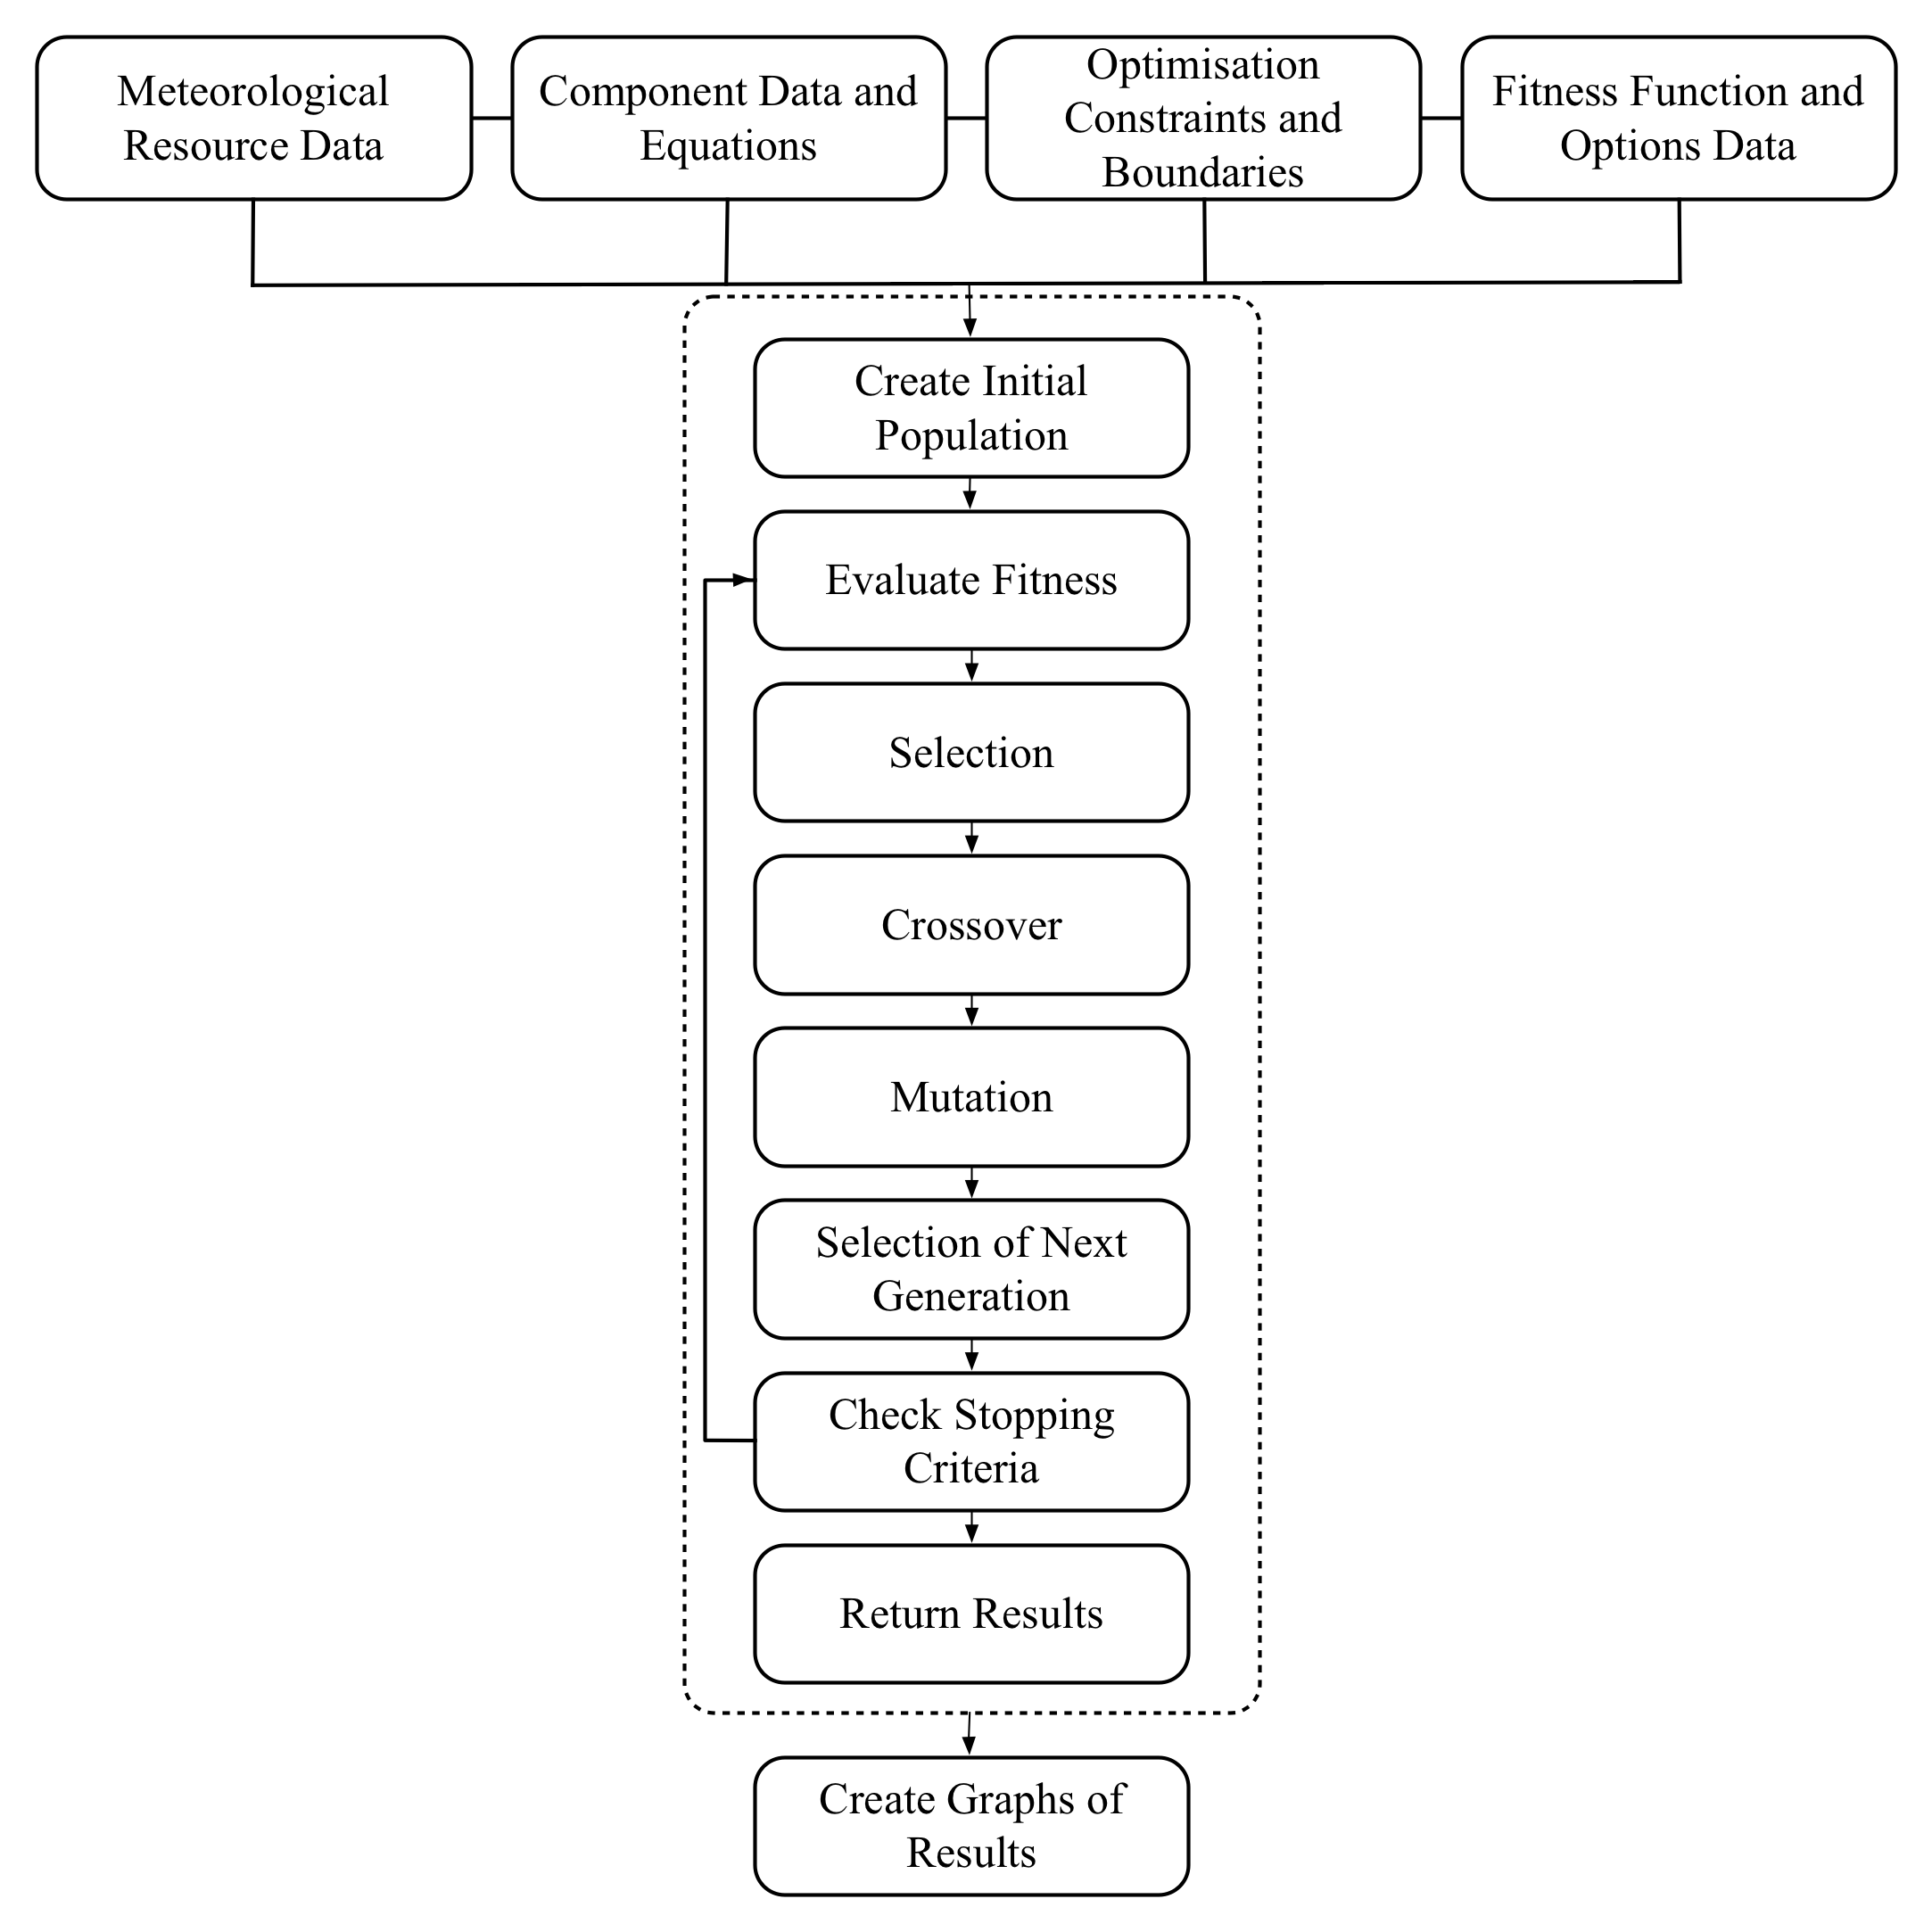
\includegraphics[width=2\columnwidth]{Figures/FlowChart.png}
\begin{small}
\onecolumn
\textbf{Appendix A:} Flowchart for the genetic algorithm used to optimise the system. Resource and component data are input alongside constraints, boundaries, fitness function and options data. The Genetic algorithm (indicated within the dashed lines) is then implemented to develop the optimised before the output in graphical format.
\label{fiowChart}
\end{small}
\twocolumn

\clearpage
\bibliographystyle{model1-num-names}
\bibliography{References/Bibliography.bib}

\end{document}